\subsection{Test Journal: Component models} \label{app:tj_0}

\textbf{Executed by: Kasper} \\
\textbf{Date: 10/5/2022}

\subsubsection*{Objective}
This test aims to document the behavior of the component models defined in \cref{sec:reformulation-of-components}.

\subsubsection*{Background}
In the plots in \cref{sec:model-verification} the states $ M_{pjj} $ and $ M_{con} $ seemed to be integrating. This indicated that the component models were not connected in an appropriate way.
Additionally in the B matrix of the linearised system, found in \cref{eq:B}, the system also showed that the compressor speed and the condenser throttle valve opening degree did not affect the states of interest, which further indicates that the non linear model could be flawed.
Before connecting all the components into one big new system, an intermediate step will be introduced. This is a verification of all of the individual component models.


\subsubsection*{Test subject}
The test subjects are the classes
\begin{itemize}
	\item boxModel
	\item compressorModel
	\item condenserModel
	\item evaporatorModel
	\item flashtankModel
	\item pjjModel
	\item valveModel
\end{itemize}
All the components are based on the models defined in \cref{sec:mod_comp_mod}. Some of them are modified with changes defined in \cref{sec:reformulation-of-components}.\\

The following components are implemented according to \cref{sec:mod_comp_mod}.
\begin{itemize}
	\item boxModel
	\item compressorModel
	\item condenserModel
	\item evaporatorModel
\end{itemize}

The following components are modified completely according to \cref{sec:reformulation-of-components}:

\begin{itemize}
	\item flashtankModel
	\item pjjModel
	\item valveModel
\end{itemize}

The aim is to test the components before more states are introduced, in order to not introduce extra complexities before a the simplest models are confirmed. This also means that the extra states in the condenser and evaporator is not tested in this test.


\subsubsection*{Equipment used}
The outputs from a simulation of "eTRU\_prototype\_2\_old\_perhabs\_with\_measurements.slx" are used as inputs for the test. The imported data can be found in "HiFi\_model\_data\_for\_component\_tests\_03.mat".
The script used for the tests are to be found in "componentModelTesting.m". with support from testinit.m.
All the files can be found in the git repository under CA8Project/Modeling/ComponentSimulation with the commit hash 25682de26edbdb141551d64b280ee66e48e26d2e.

\subsubsection*{Test setup}
The component models are compared to the HiFi simulation. This means that the measurements that are inputs to the components in the Hifi simulation model are used as inputs to the test subjects: the component models. The outputs of the test subjects are then compared with the outputs of the component models of the HiFi model.

\subsubsection*{Test procedure}
Run the script "ComponentModelTesting.m".

\clearpage
\subsubsection*{Results and Comments}
\begin{figure}[h]
	\centering
	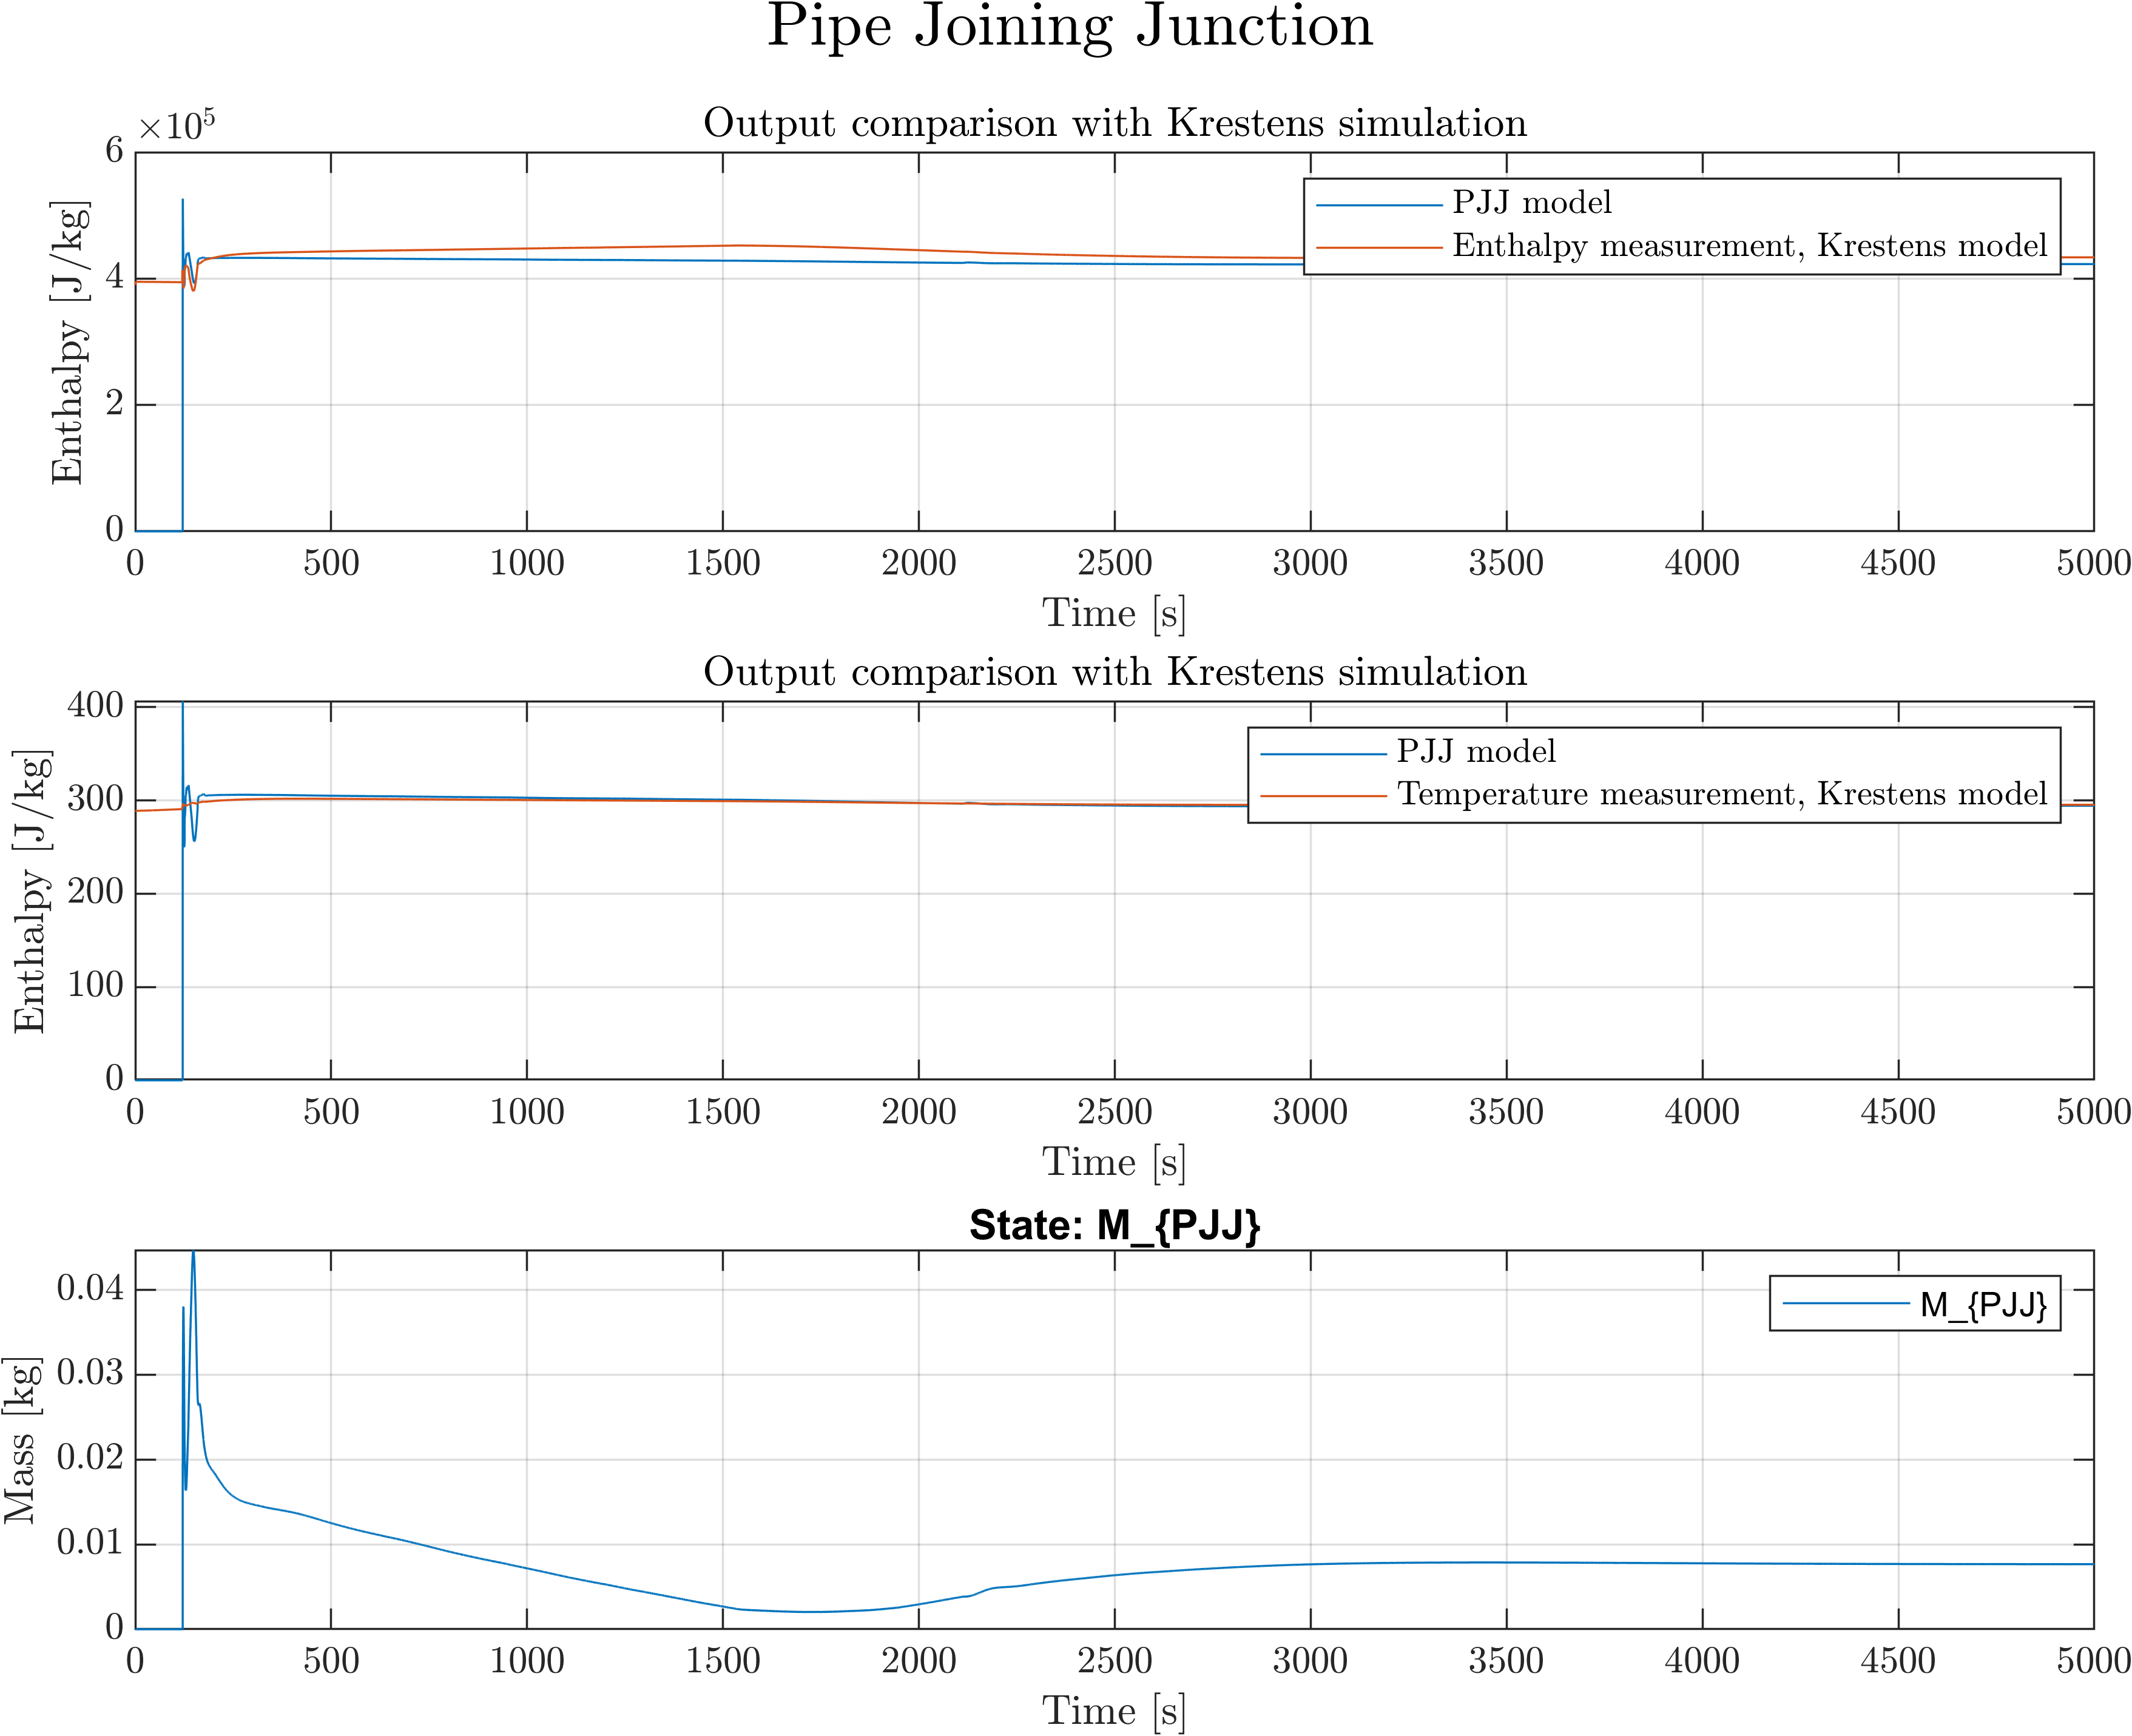
\includegraphics[width=1\textwidth]{Graphics/comp_test_box.png}
	\caption{Comparison of boxModel outputs with HiFi component model of box}
	\label{fig:component_test_box}
\end{figure}
\begin{figure}[h]
	\centering
	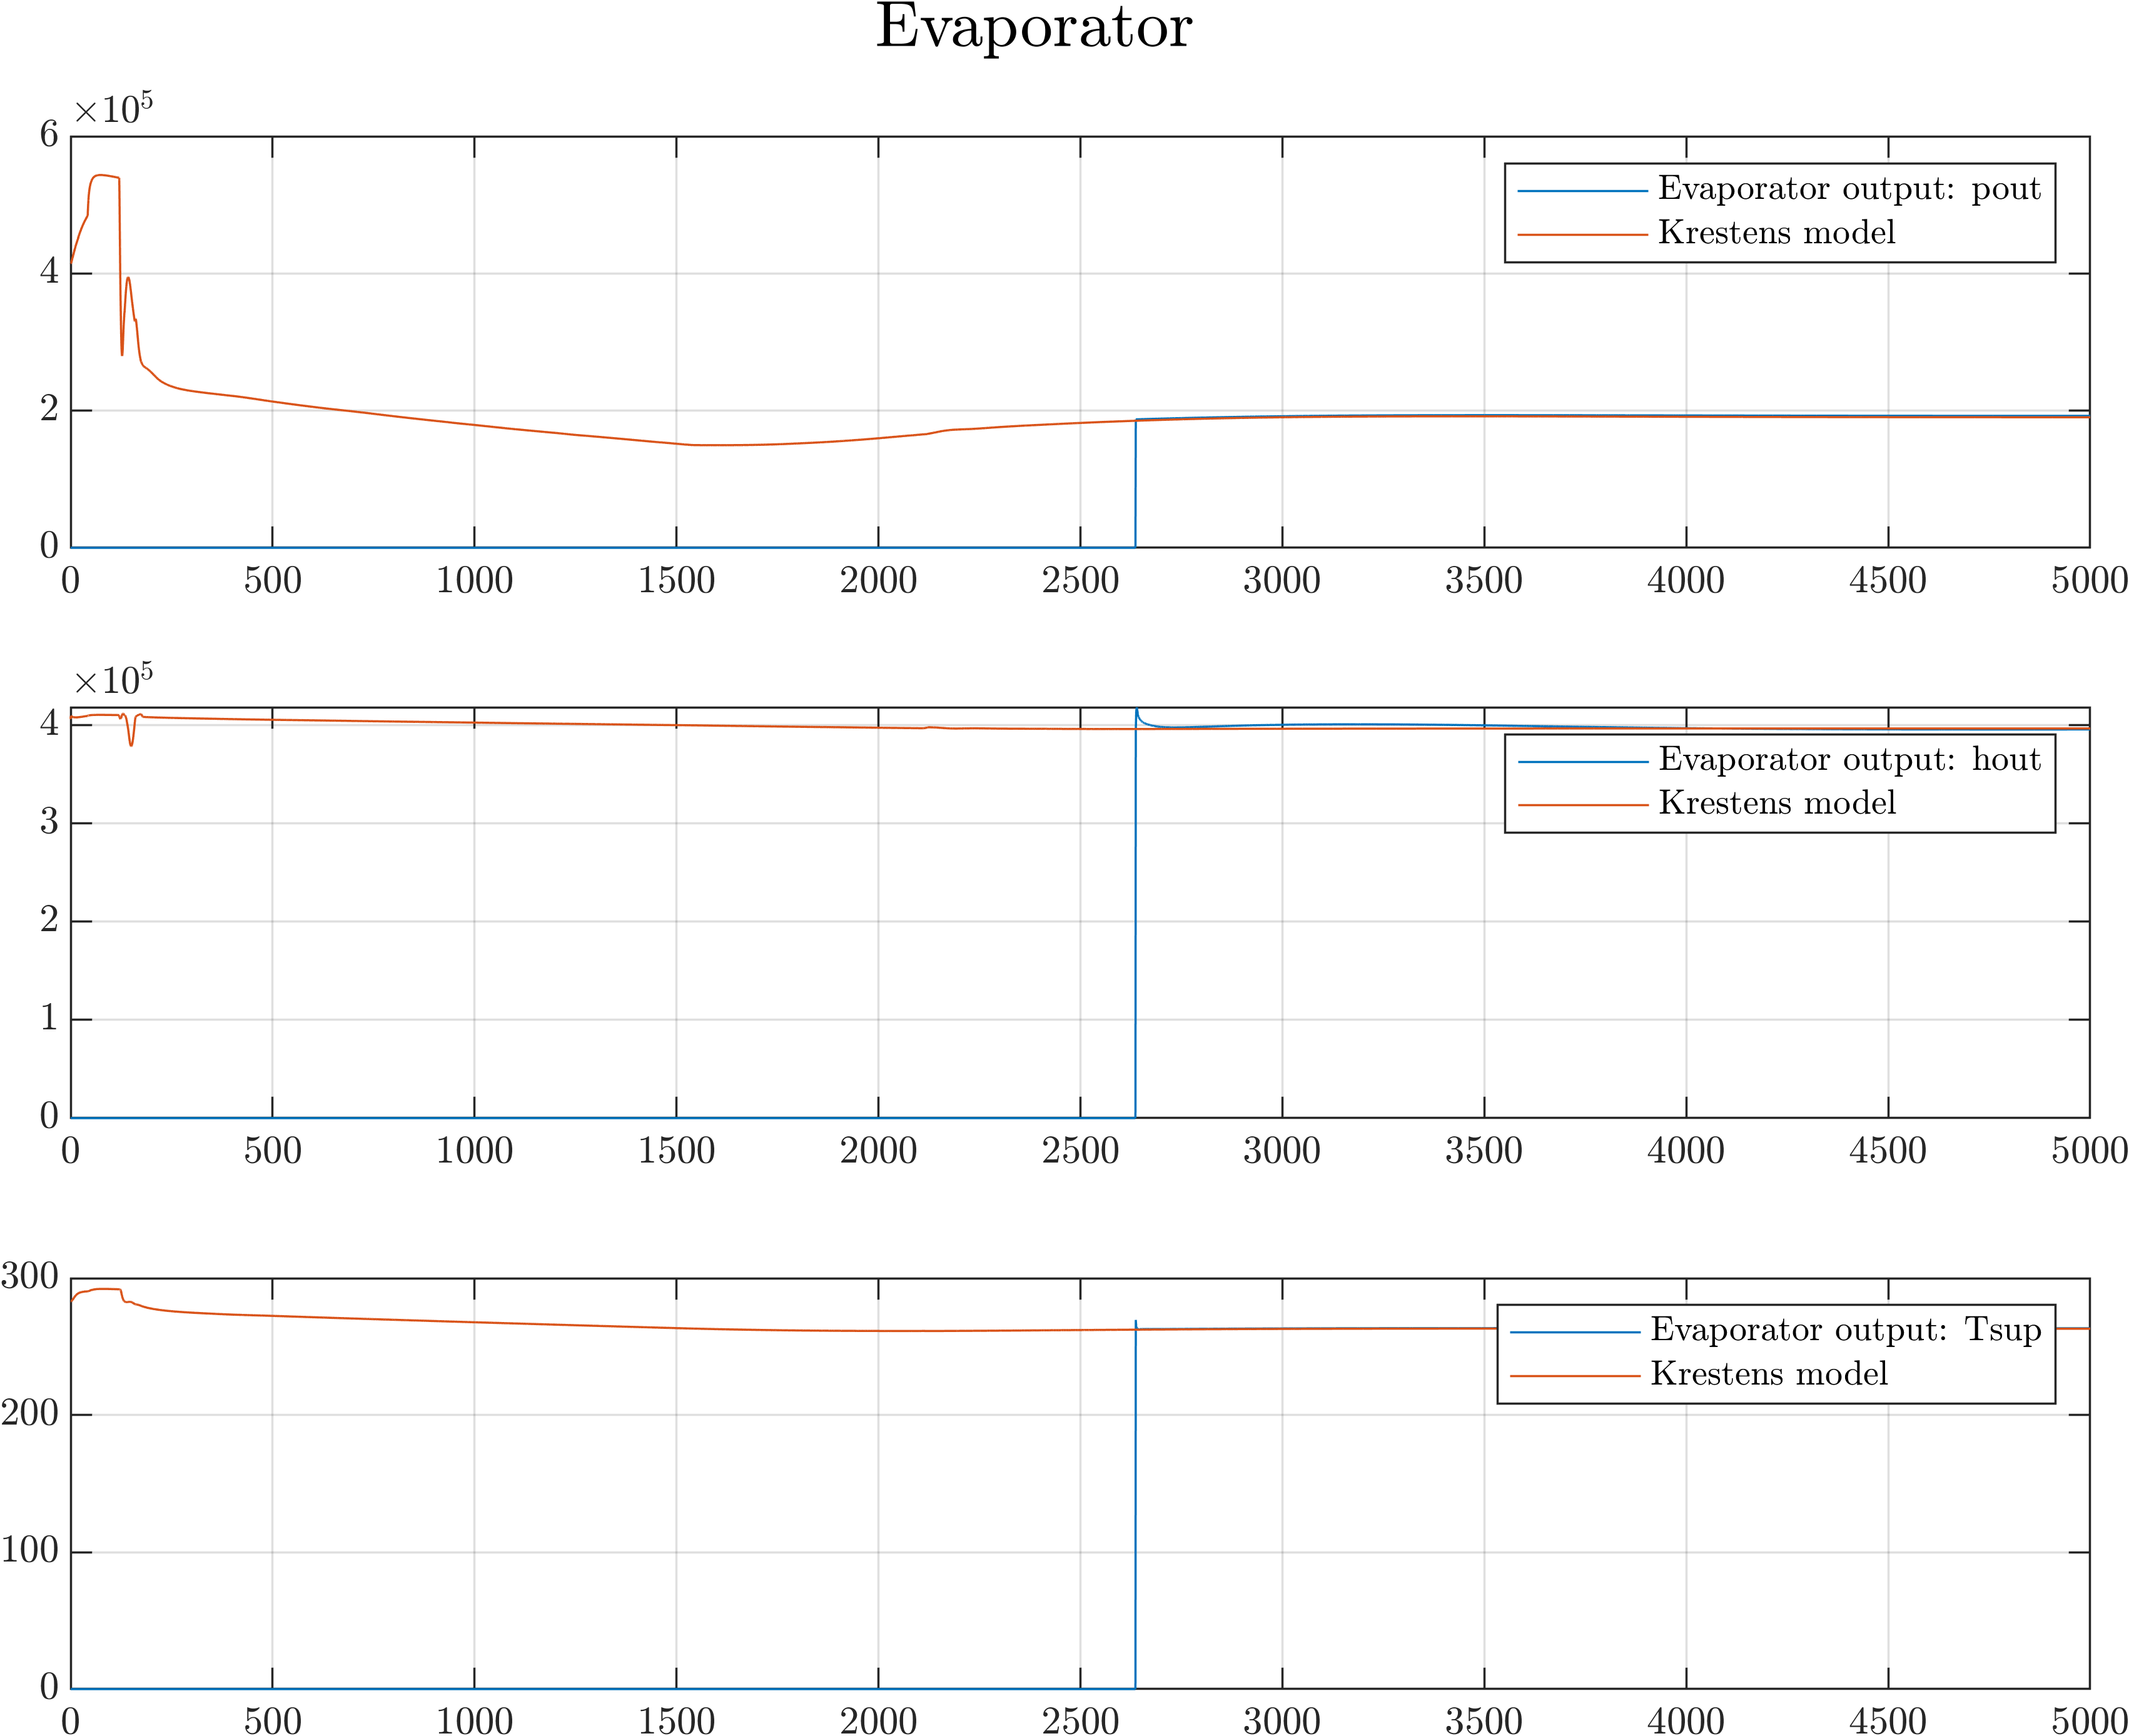
\includegraphics[width=1\textwidth]{Graphics/comp_test_com.png}
	\caption{Comparison of compressorModel outputs with HiFi component model of compressor}
	\label{fig:component_test_com}
\end{figure}
\begin{figure}[h]
	\centering
	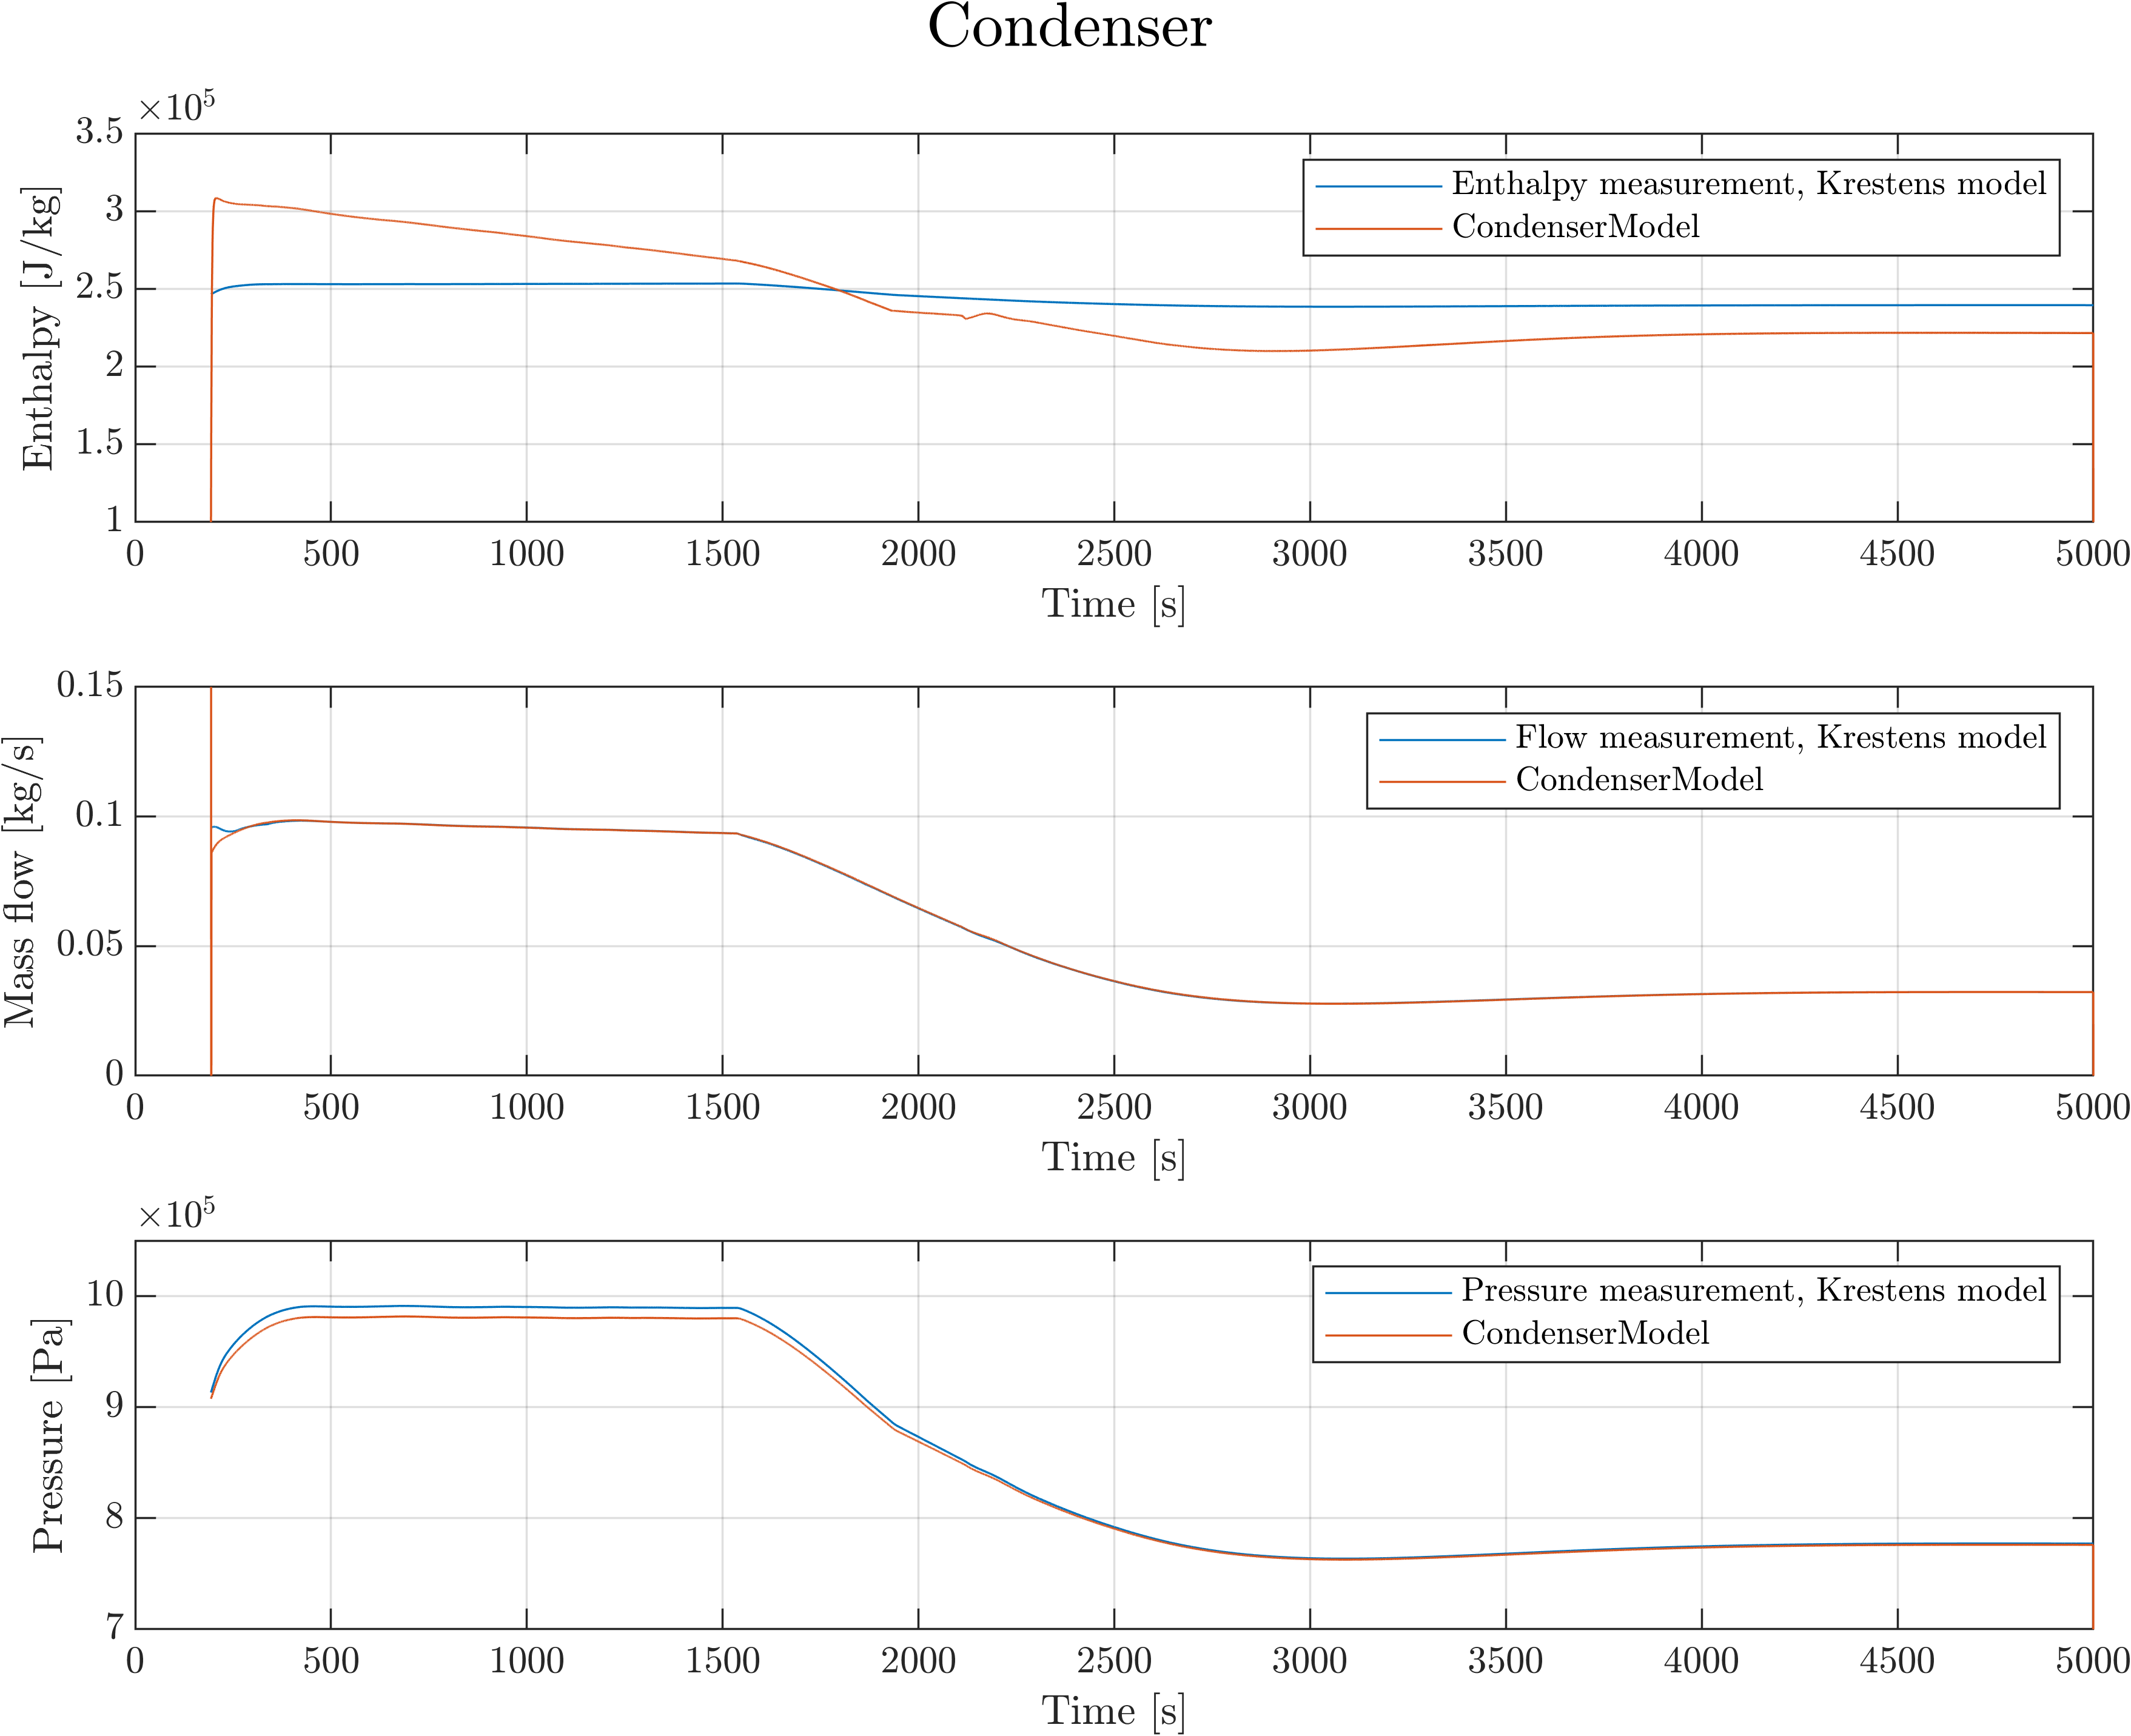
\includegraphics[width=1\textwidth]{Graphics/comp_test_con.png}
	\caption{Comparison of condenserModel outputs with HiFi component model of condenser}
	\label{fig:component_test_con}
\end{figure}
\begin{figure}[h]
	\centering
	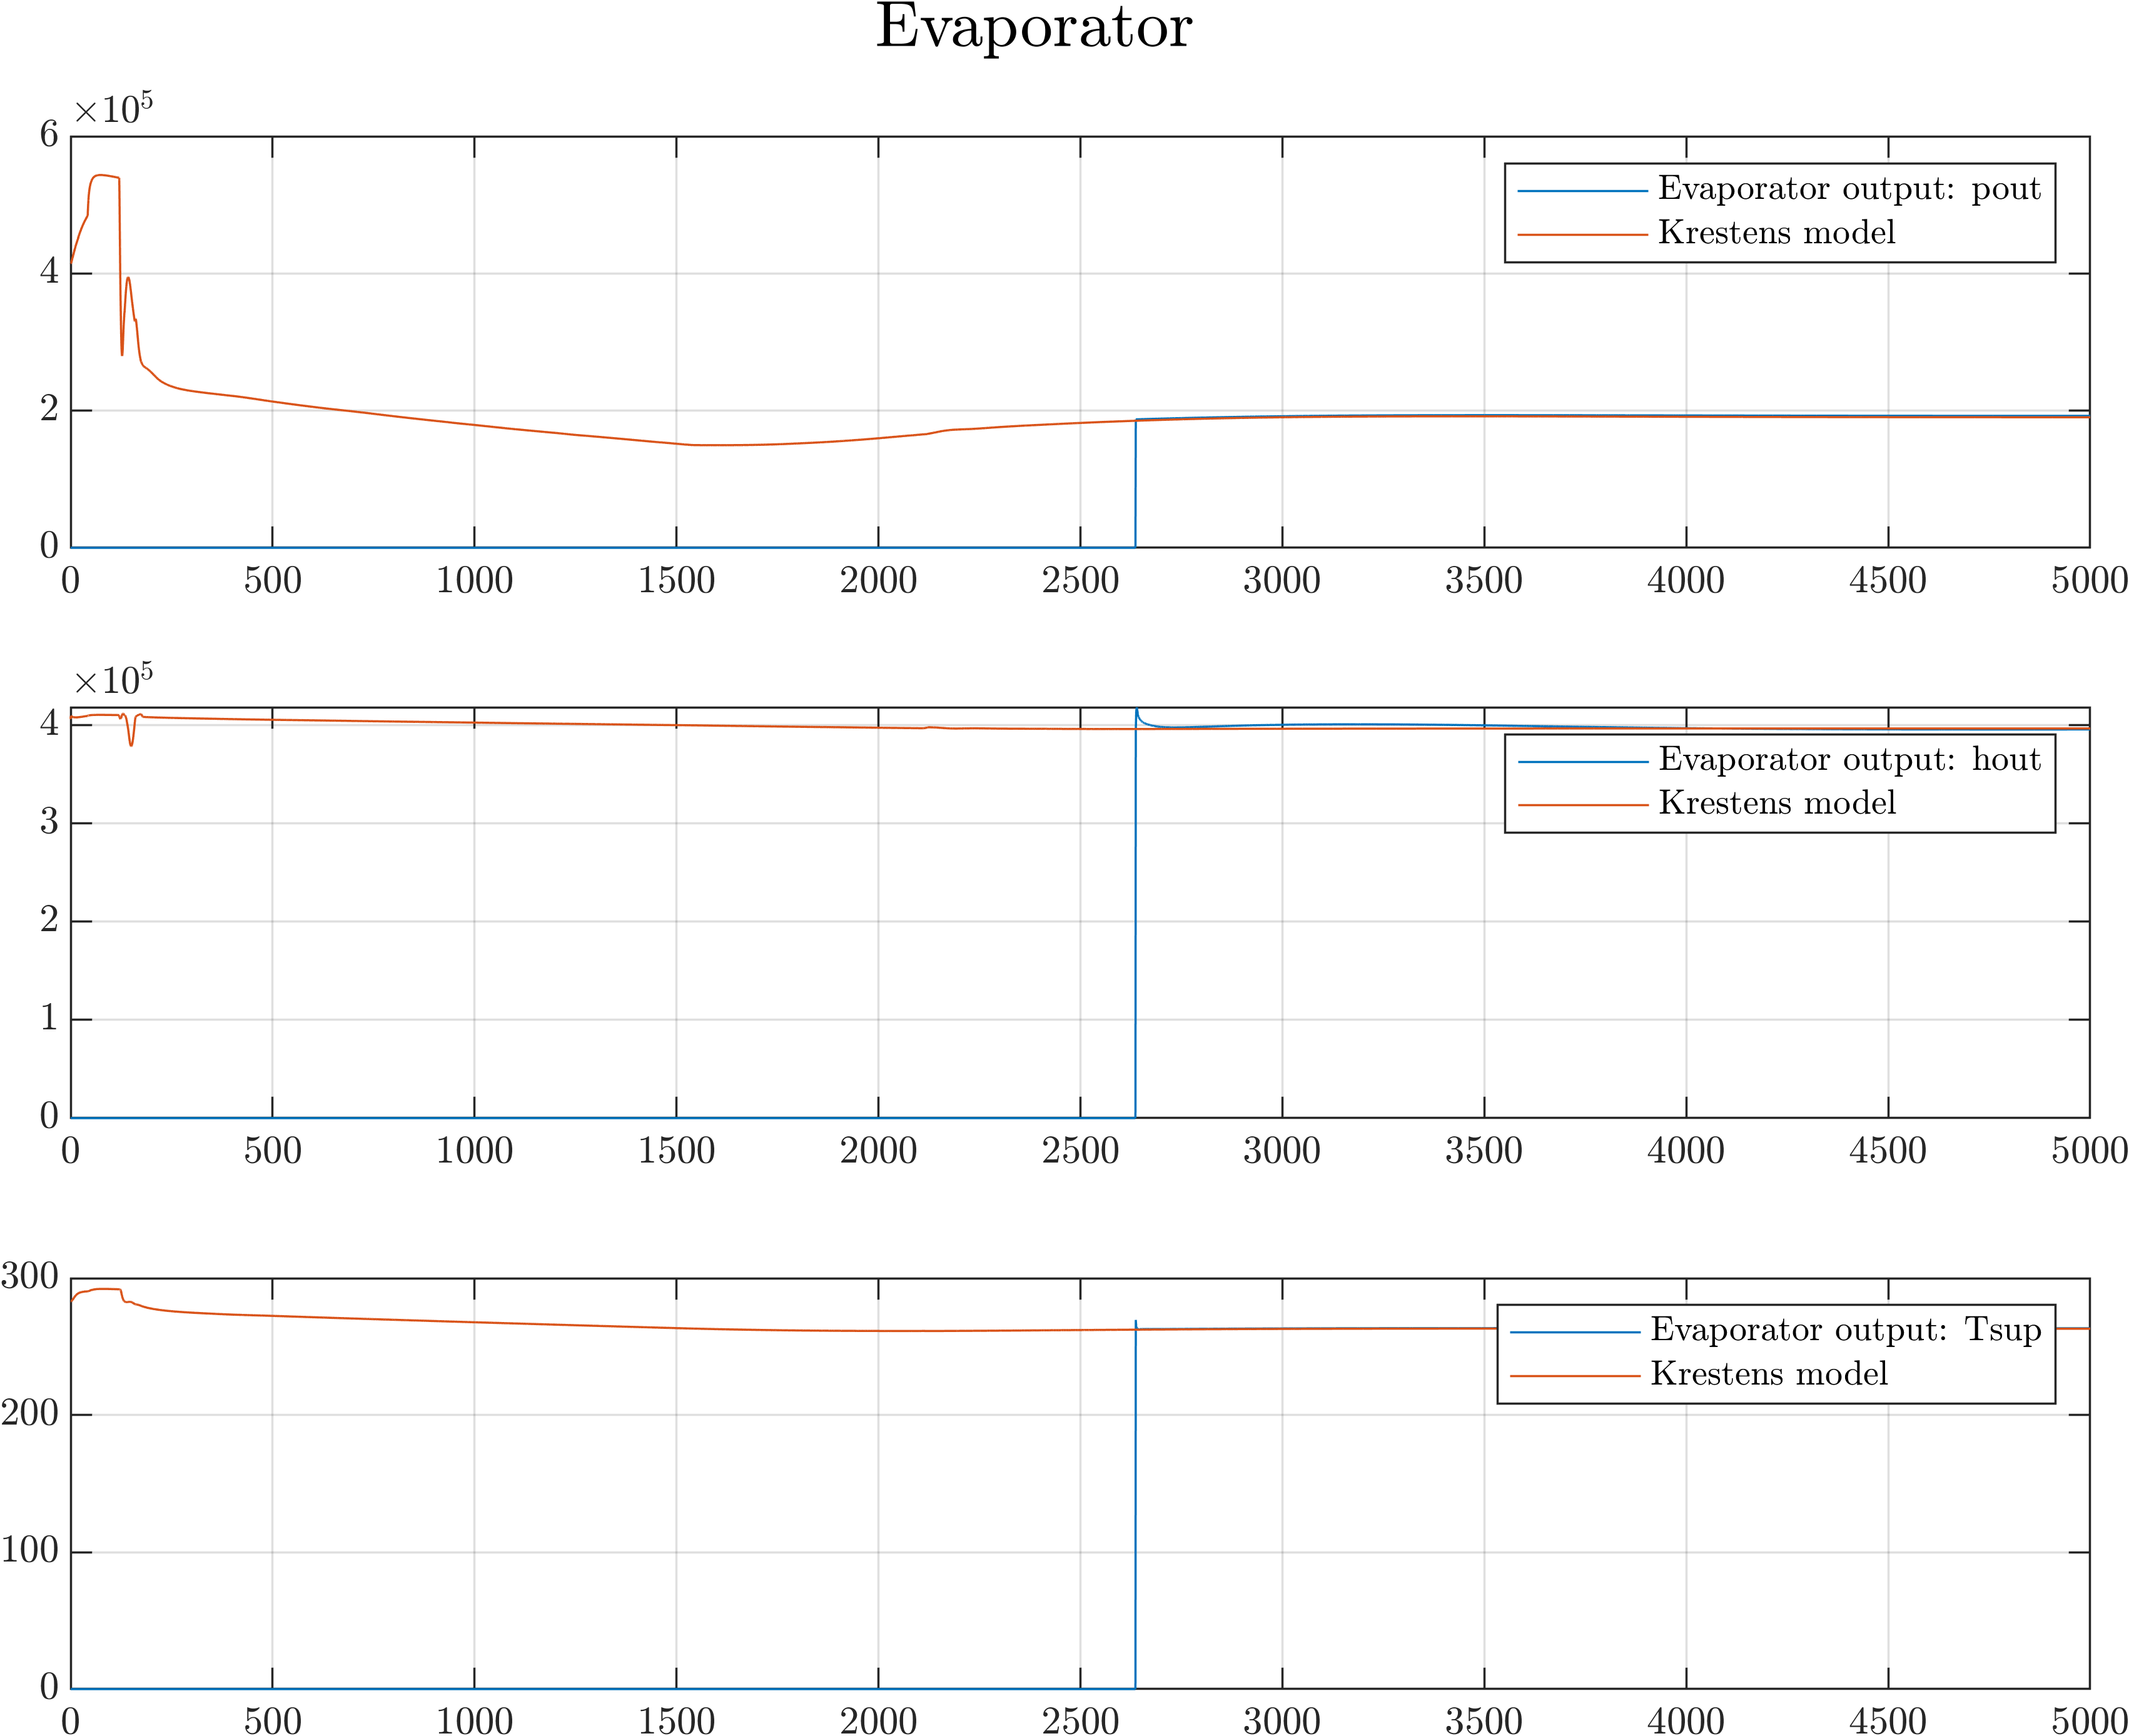
\includegraphics[width=1\textwidth]{Graphics/comp_test_eva.png}
	\caption{Comparison of evaporatorModel outputs with HiFi component model of evaporator}
	\label{fig:component_test_eva}
\end{figure}
\begin{figure}[h]
	\centering
	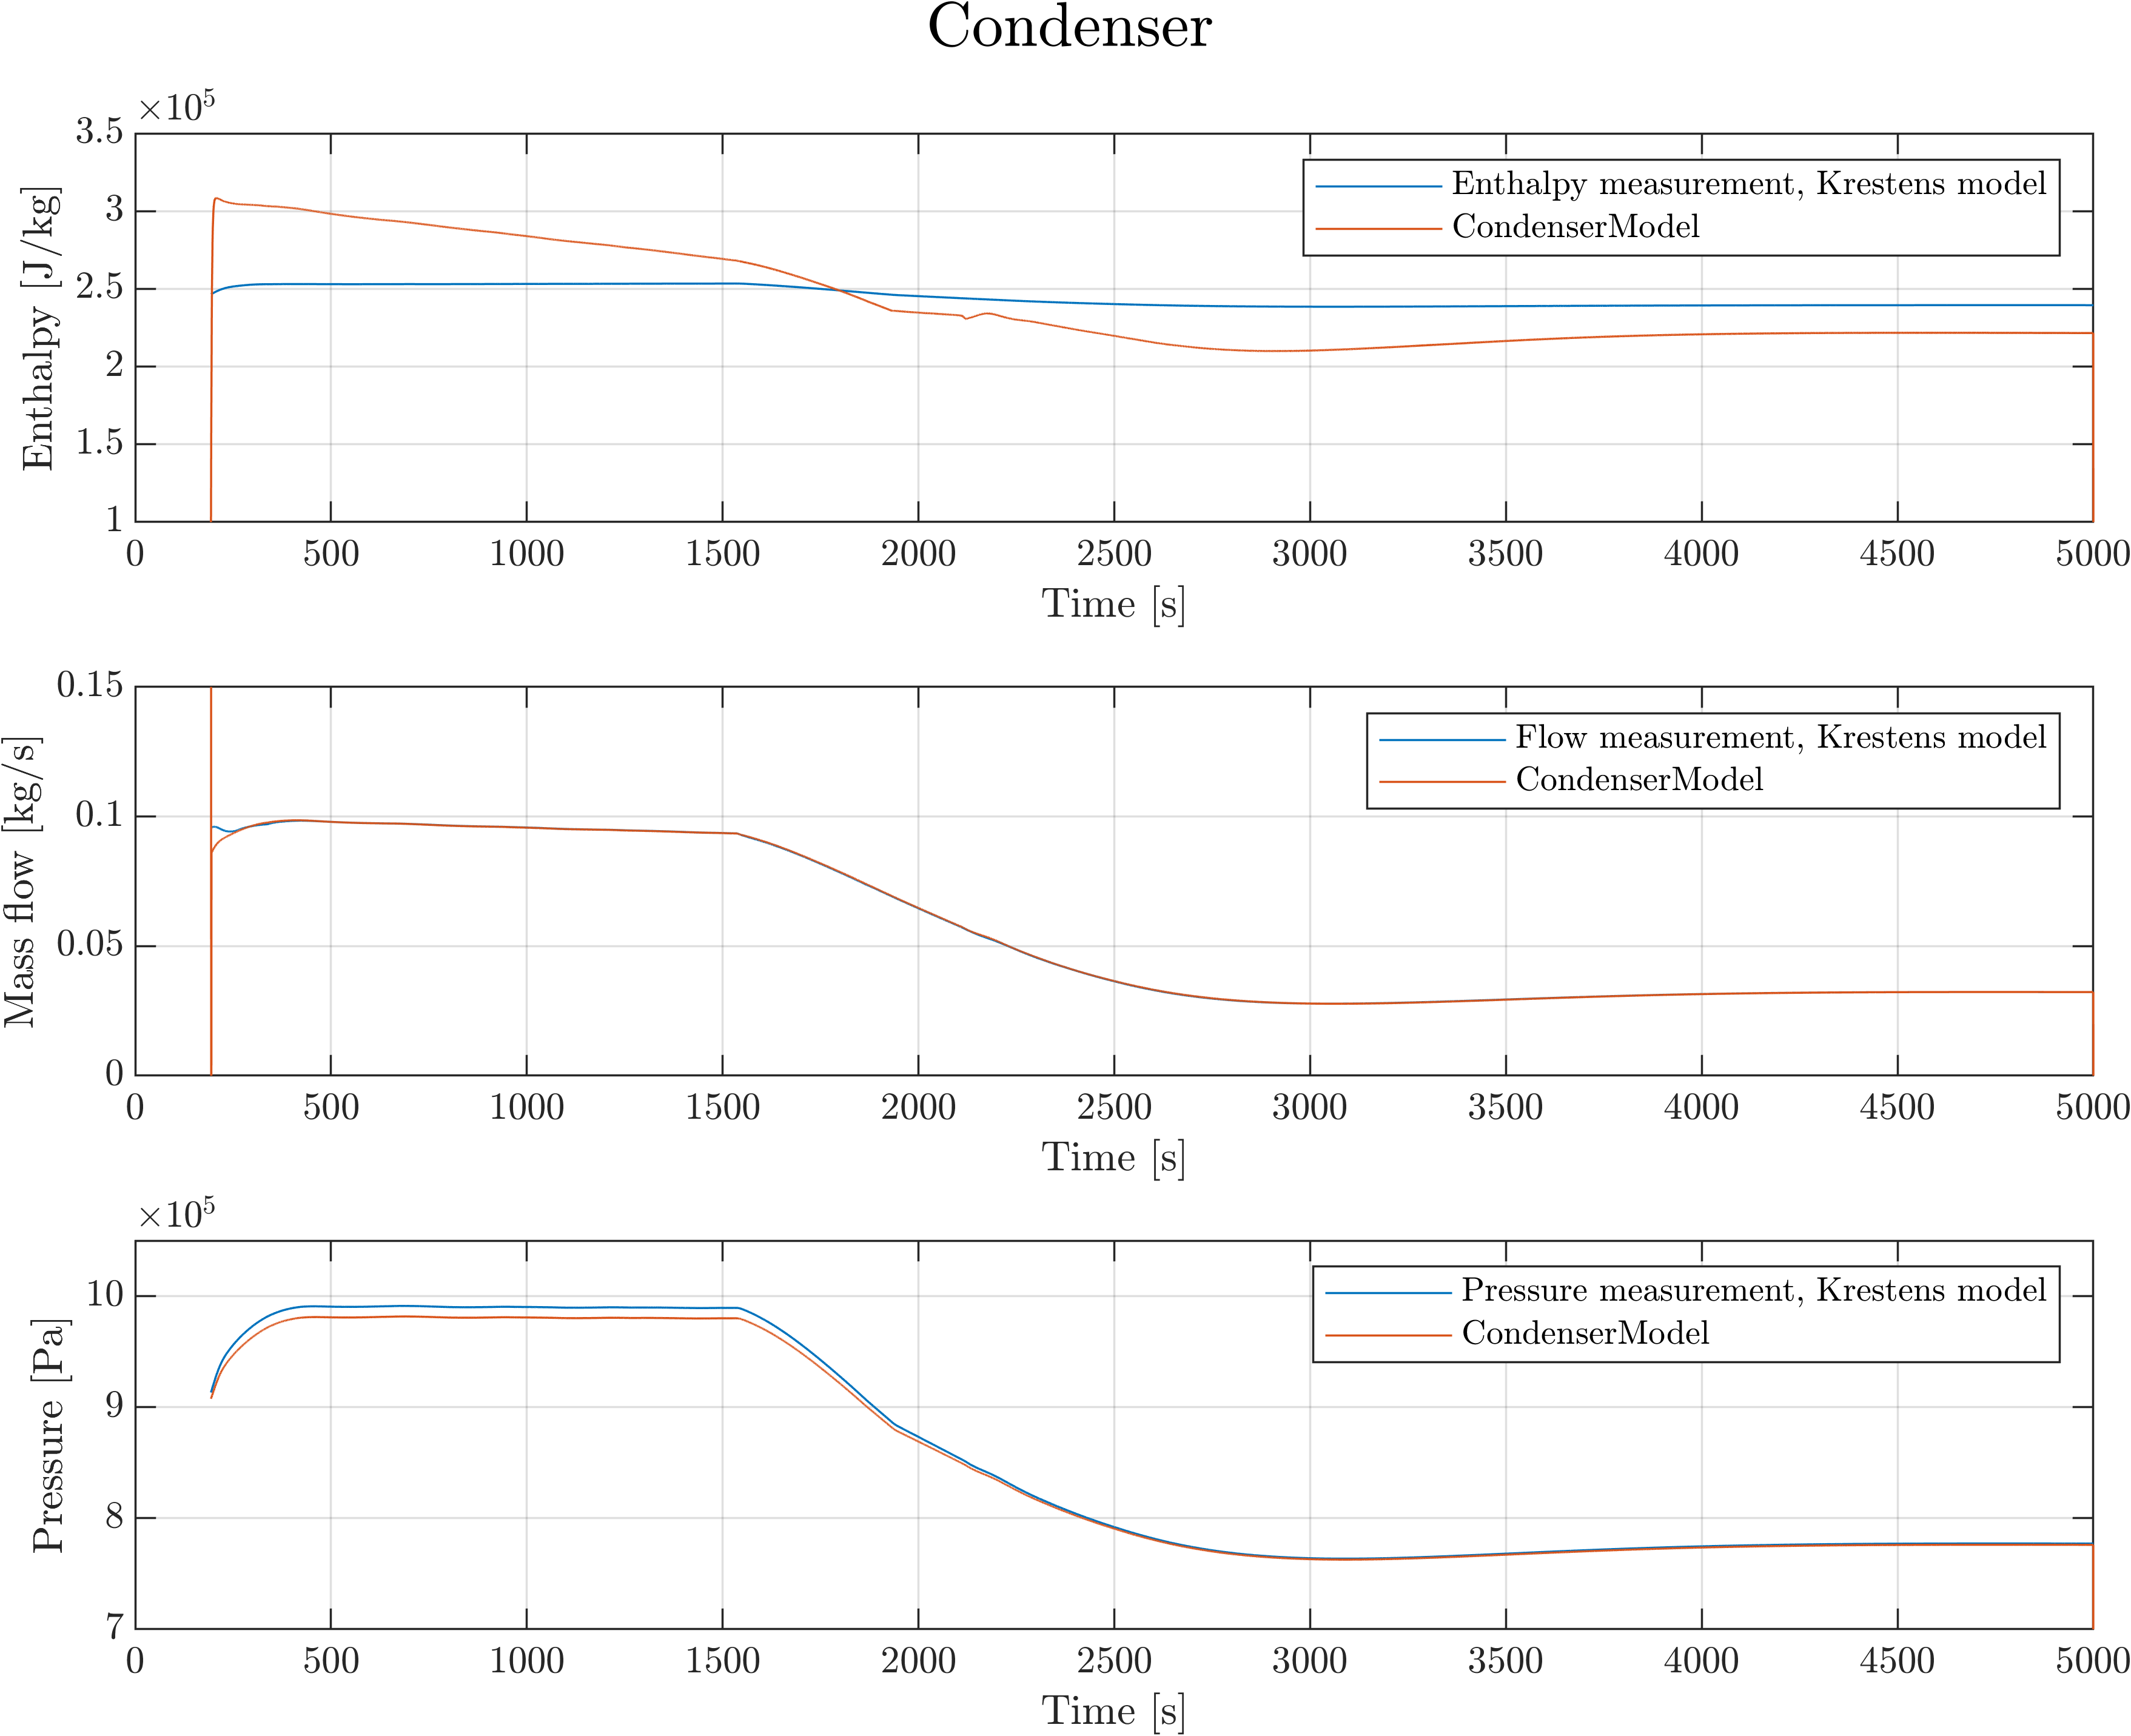
\includegraphics[width=1\textwidth]{Graphics/comp_test_ft.png}
	\caption{Comparison of flashtankModel outputs with HiFi component model of flash tank}
	\label{fig:component_test_ft}
\end{figure}
\begin{figure}[h]
	\centering
	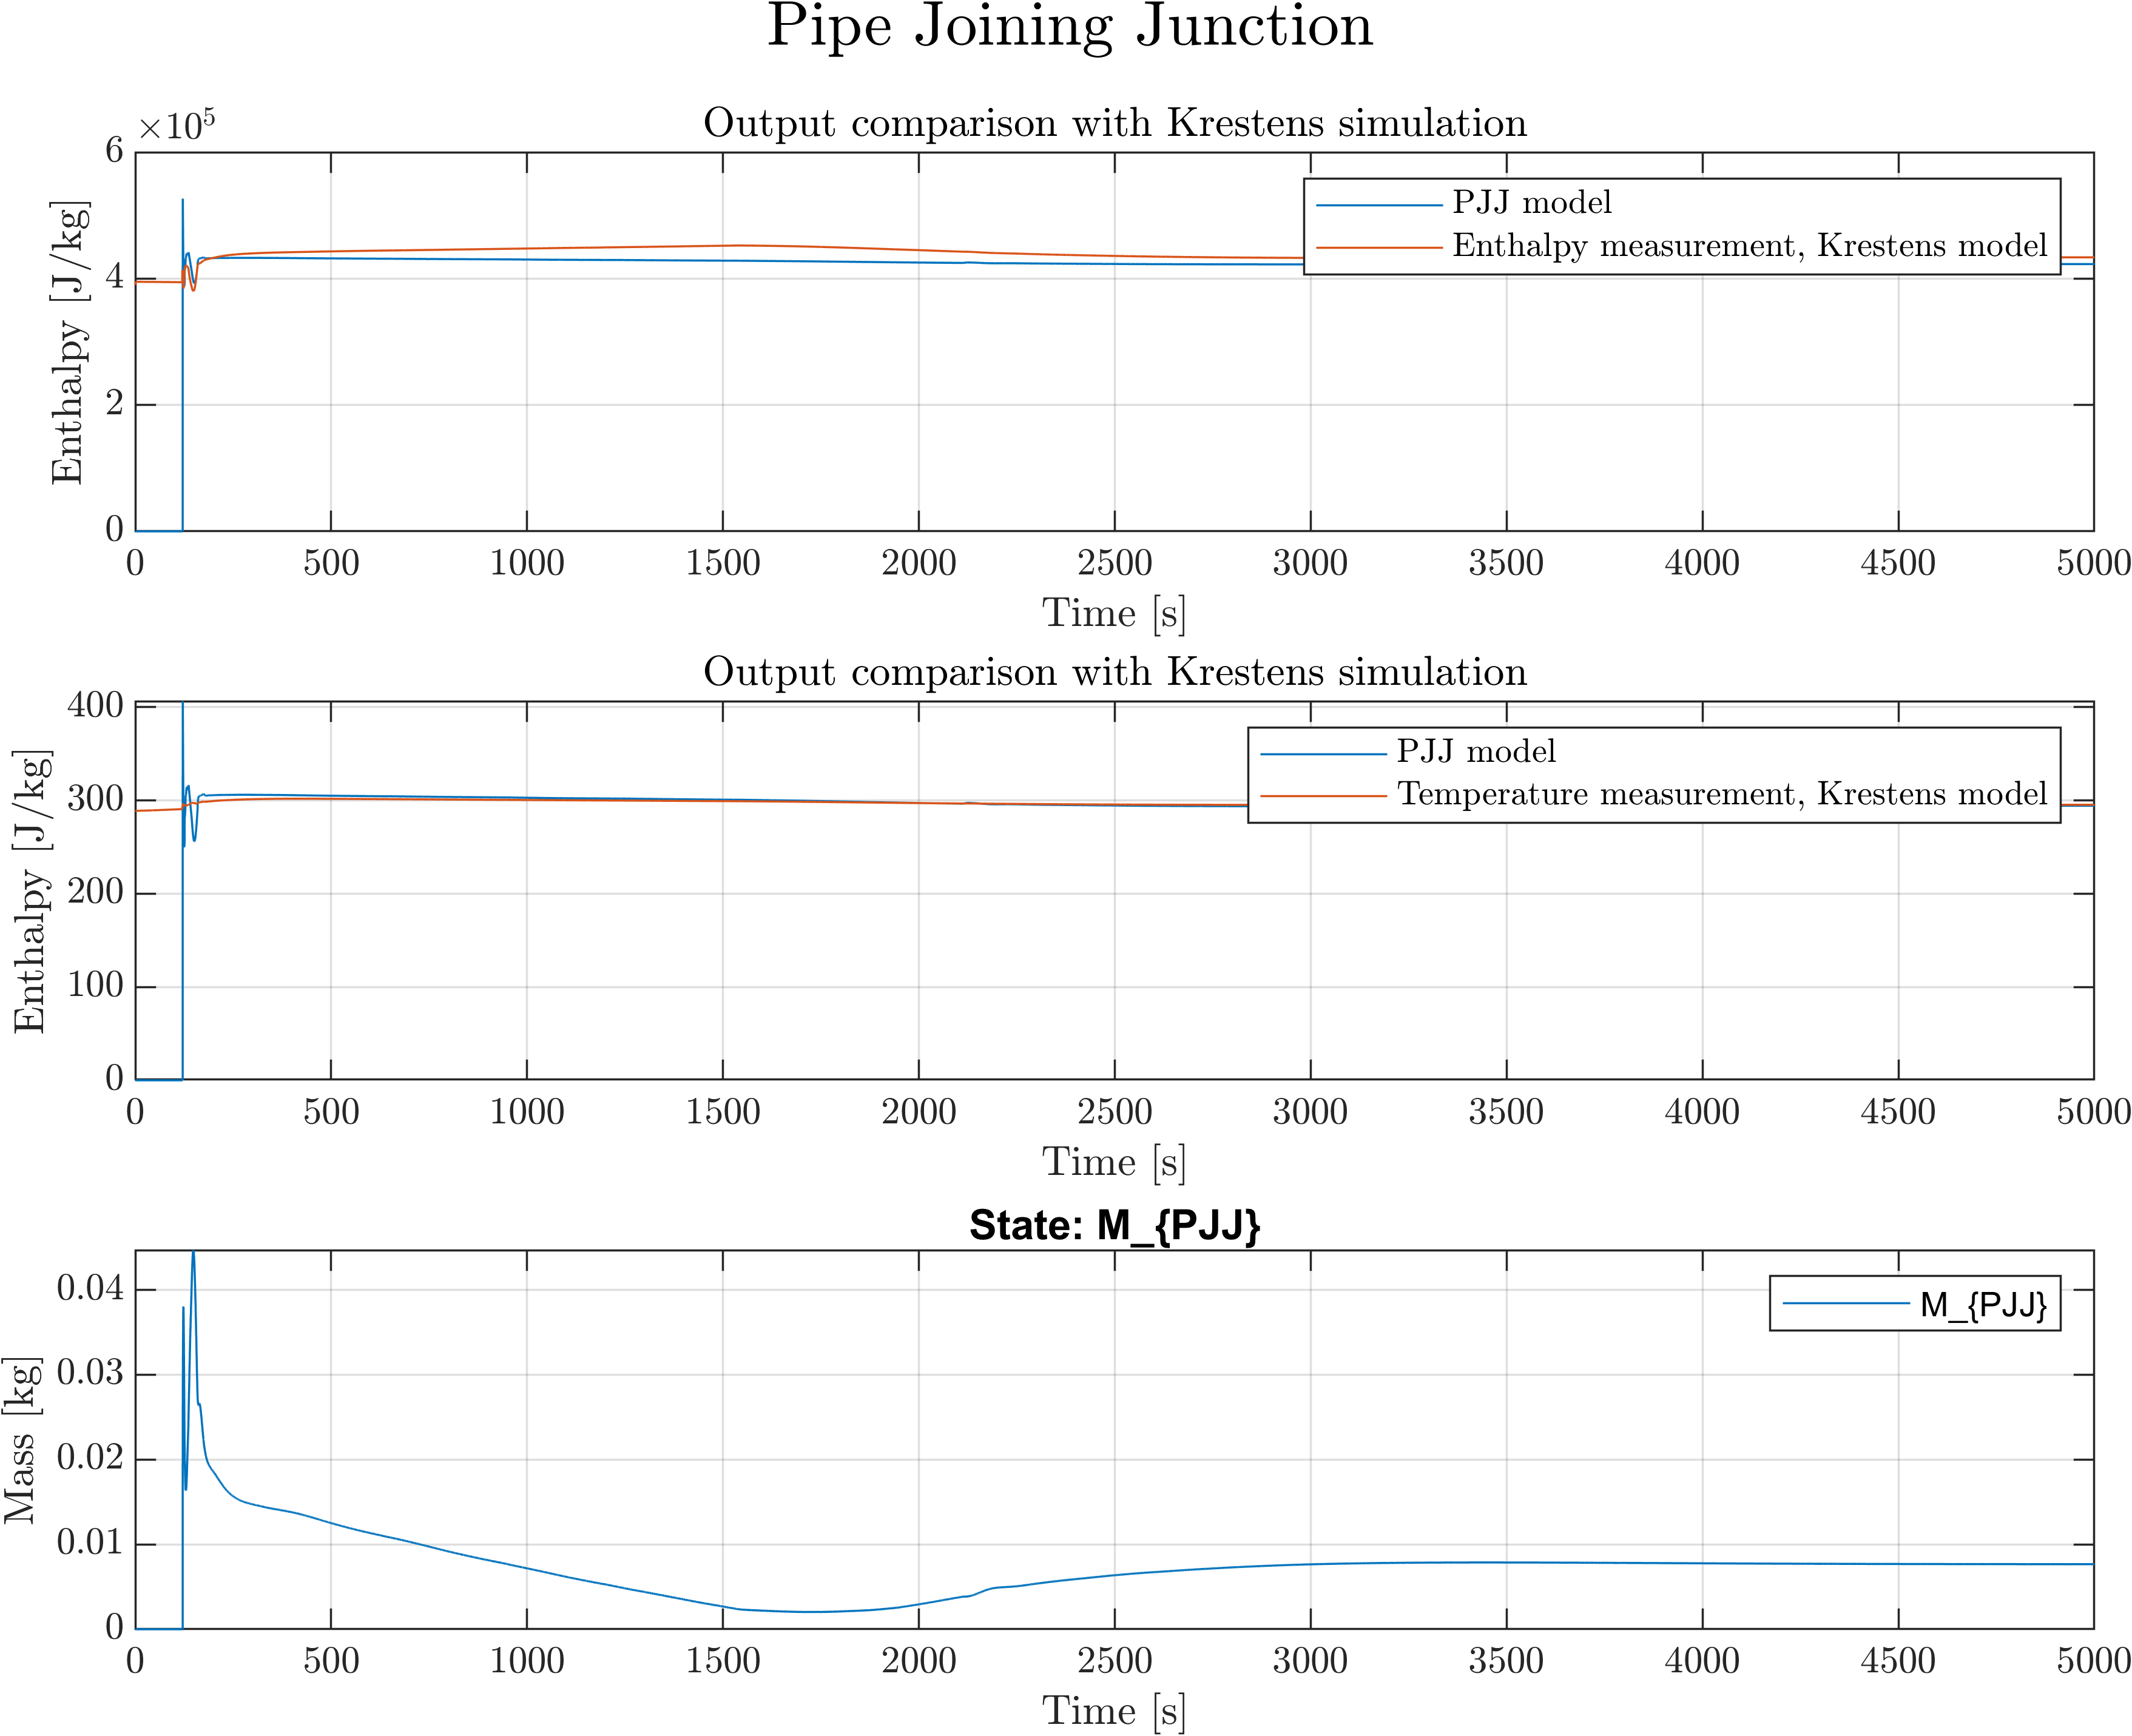
\includegraphics[width=1\textwidth]{Graphics/comp_test_pjj.png}
	\caption{Comparison of pjjModel outputs with HiFi component model of pipe joining junction}
	\label{fig:component_test_pjj}
\end{figure}
\begin{figure}[h]
	\centering
	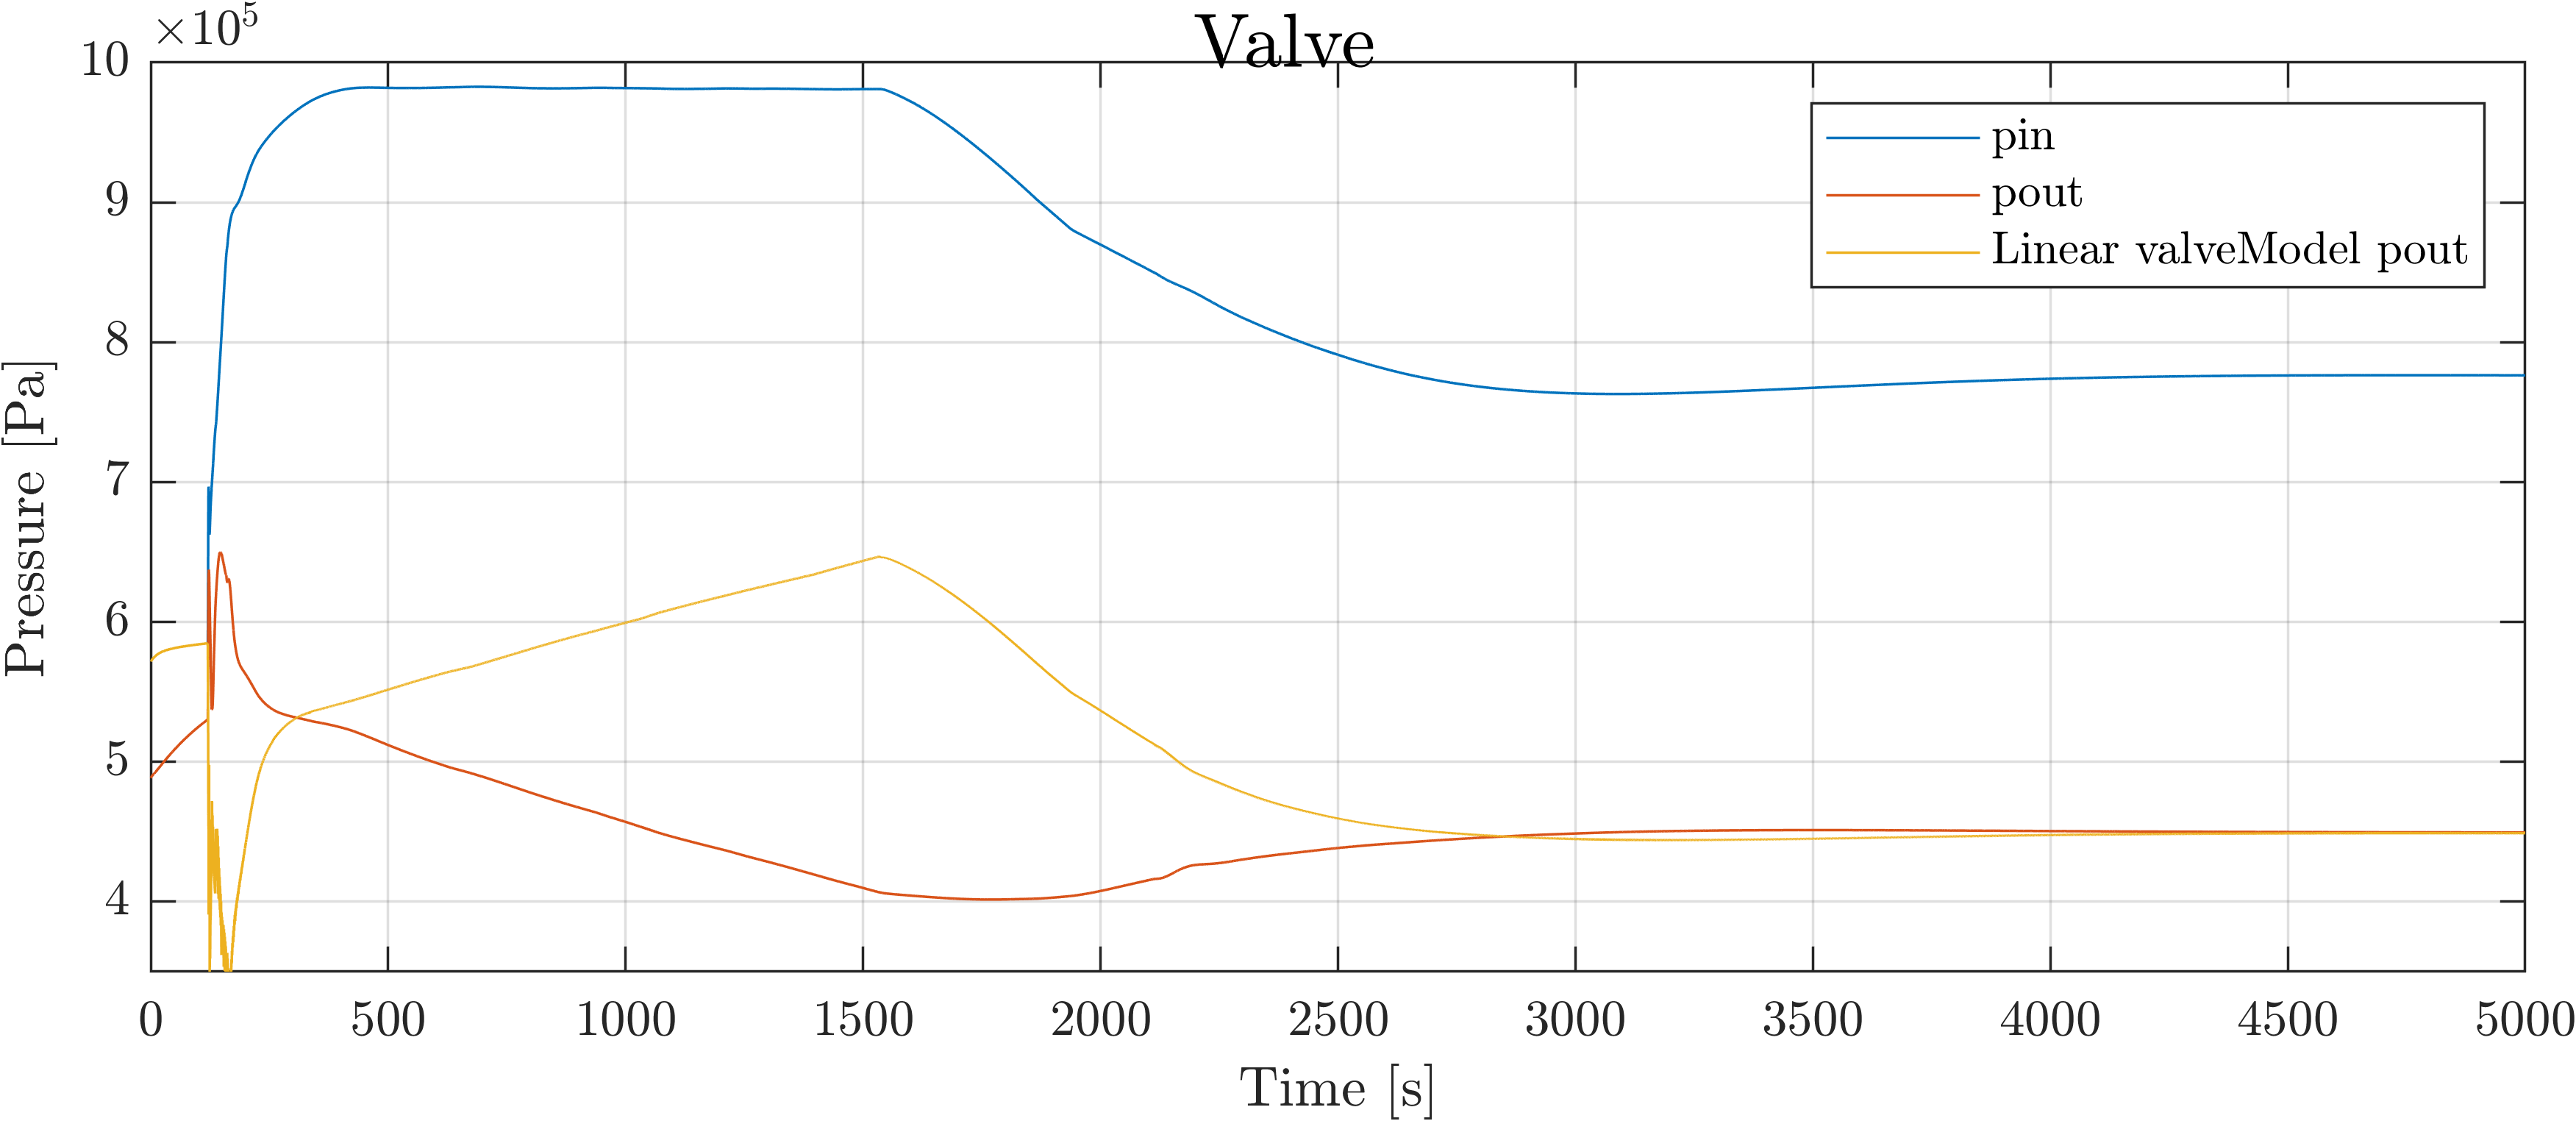
\includegraphics[width=1\textwidth]{Graphics/comp_test_val.png}
	\caption{Comparison of valveModel outputs with HiFi component model of valve}
	\label{fig:component_test_val}
\end{figure}

\clearpage
%comp_test_box.png
%comp_test_com.png
%comp_test_con.png
%comp_test_eva.png
%comp_test_ft.png
%comp_test_pjj.png
%comp_test_val.png

%First comes two plots with the output pressure being as in line 158 in \cref{fig:evapotest1_code}, \cref{fig:evapotest_plot1} showing the simulation with a start around time t= 2637 s and to the end.
%
%\begin{figure}[h]
%	\centering
%	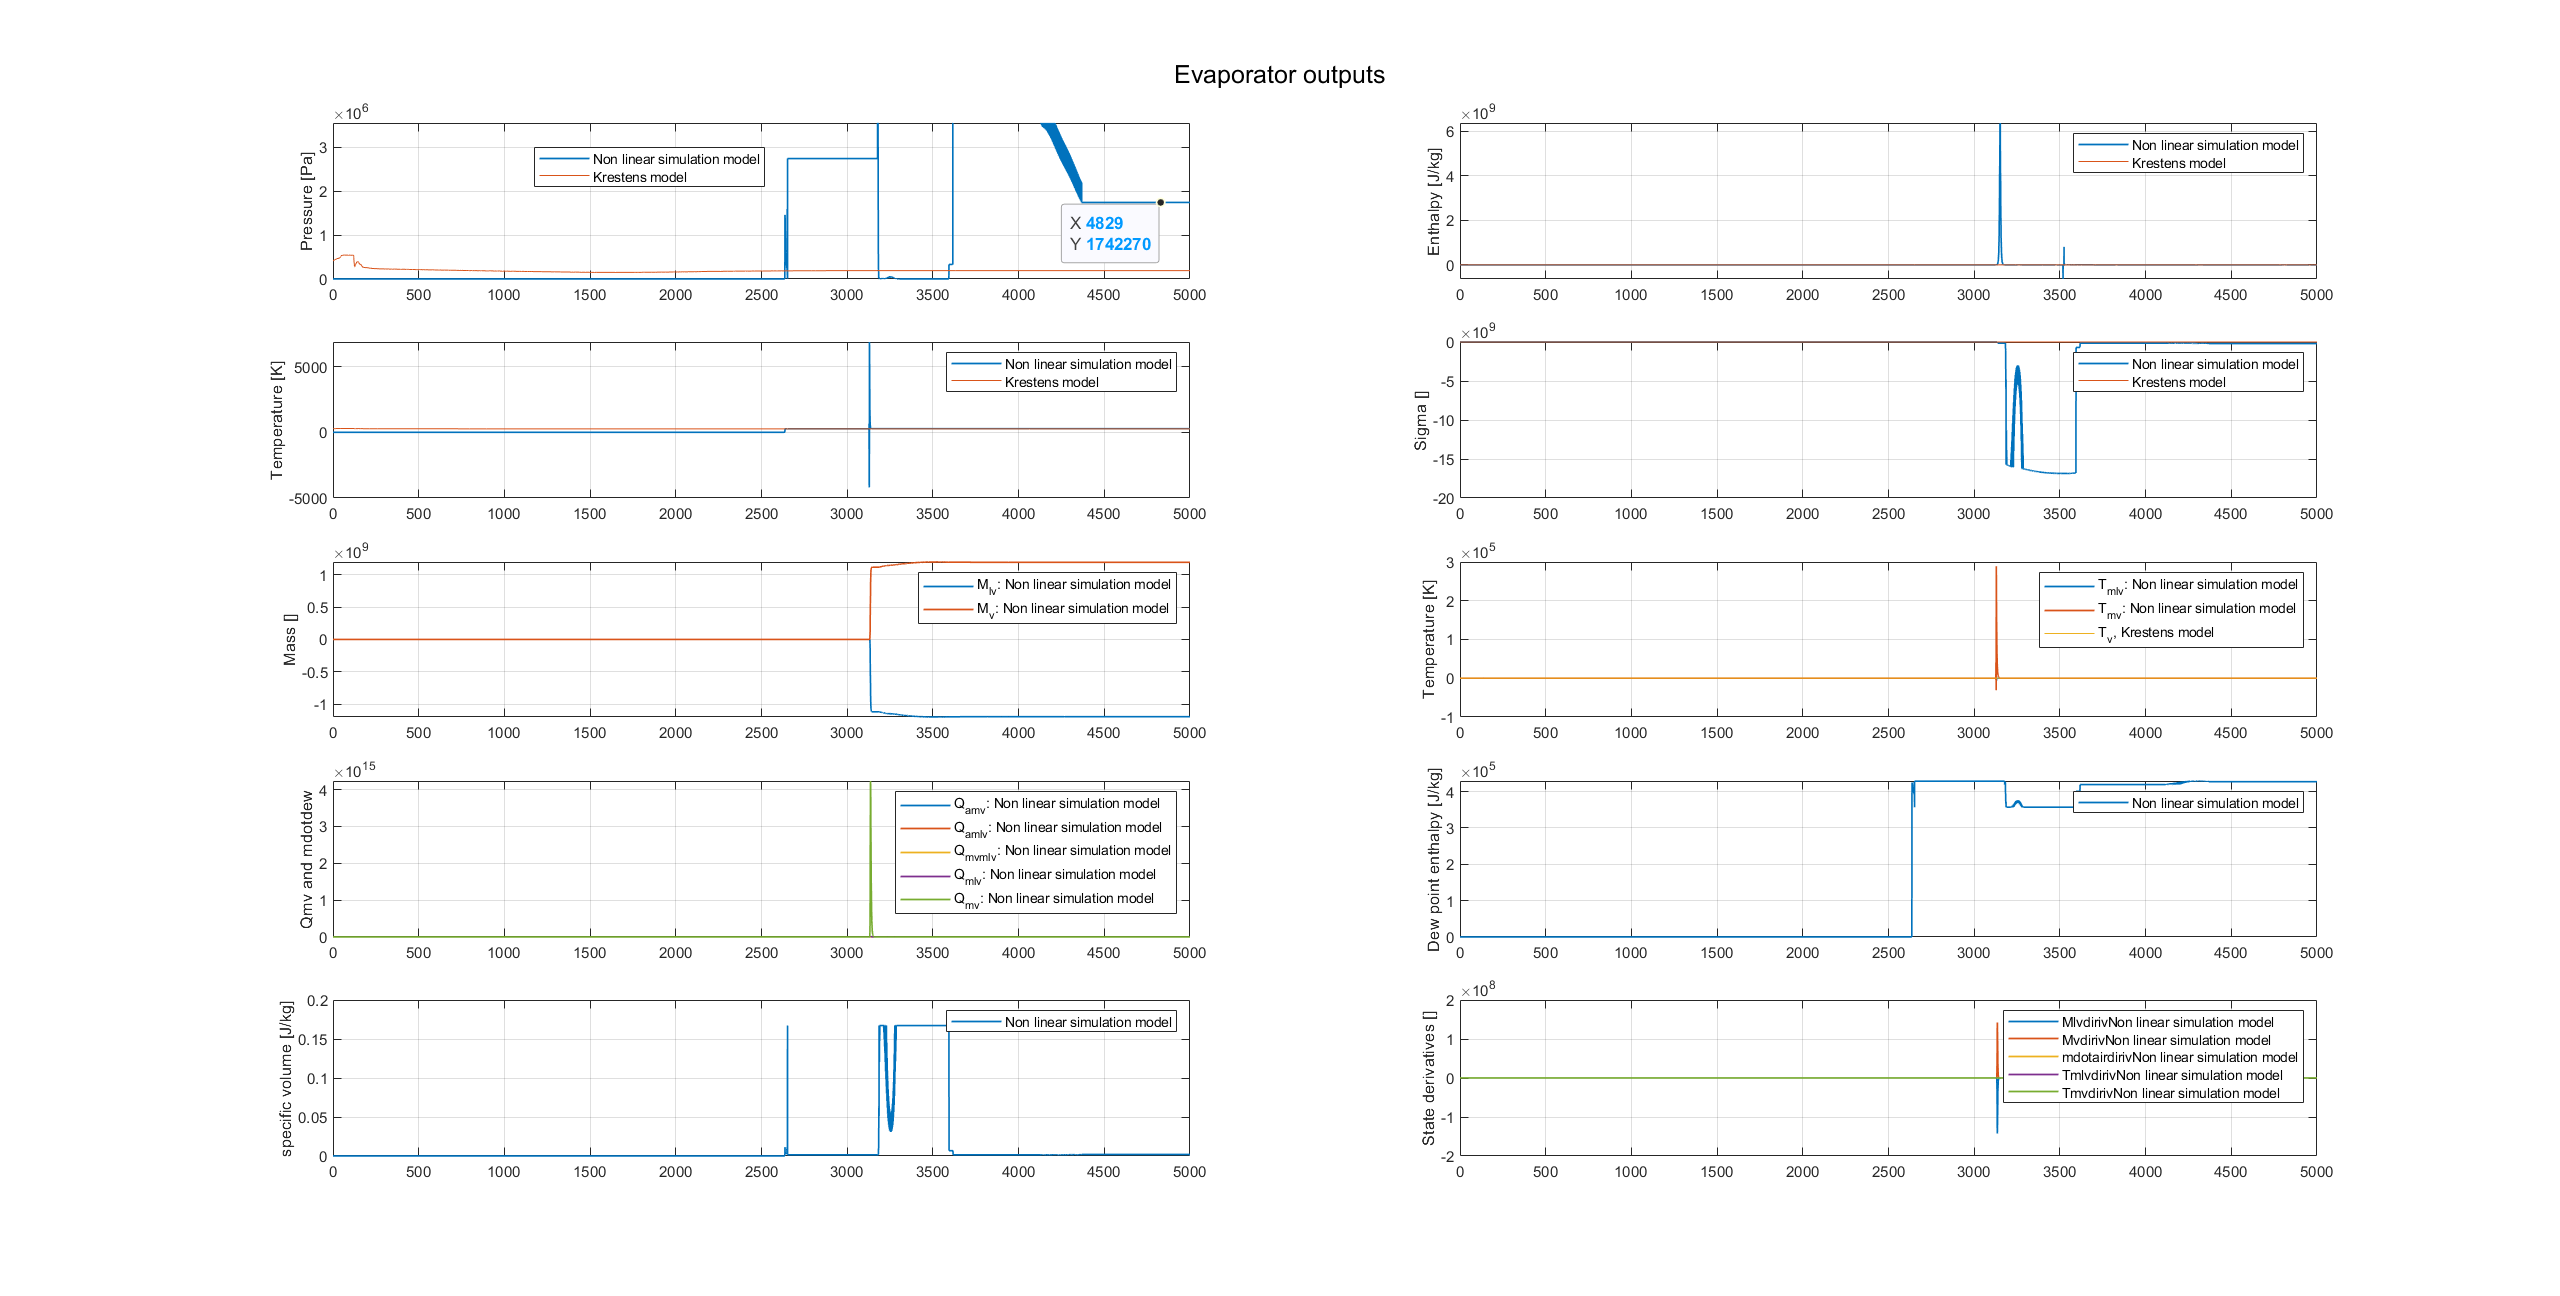
\includegraphics[width=2.1\textwidth]{Tests/Evapo_test1/plot_unstable.png}
%	\caption{Outputs with pressure out being a table lookup}
%	\label{fig:evapotest_plot1}
%\end{figure}
%
%Here if the upper left plot is observed, the output pressure of the evaporator model shows unstable behavior and eventual settling around a way to high value of 17.4 bar = 1740000 Pa.
%
%\begin{figure}[h]
%	\centering
%	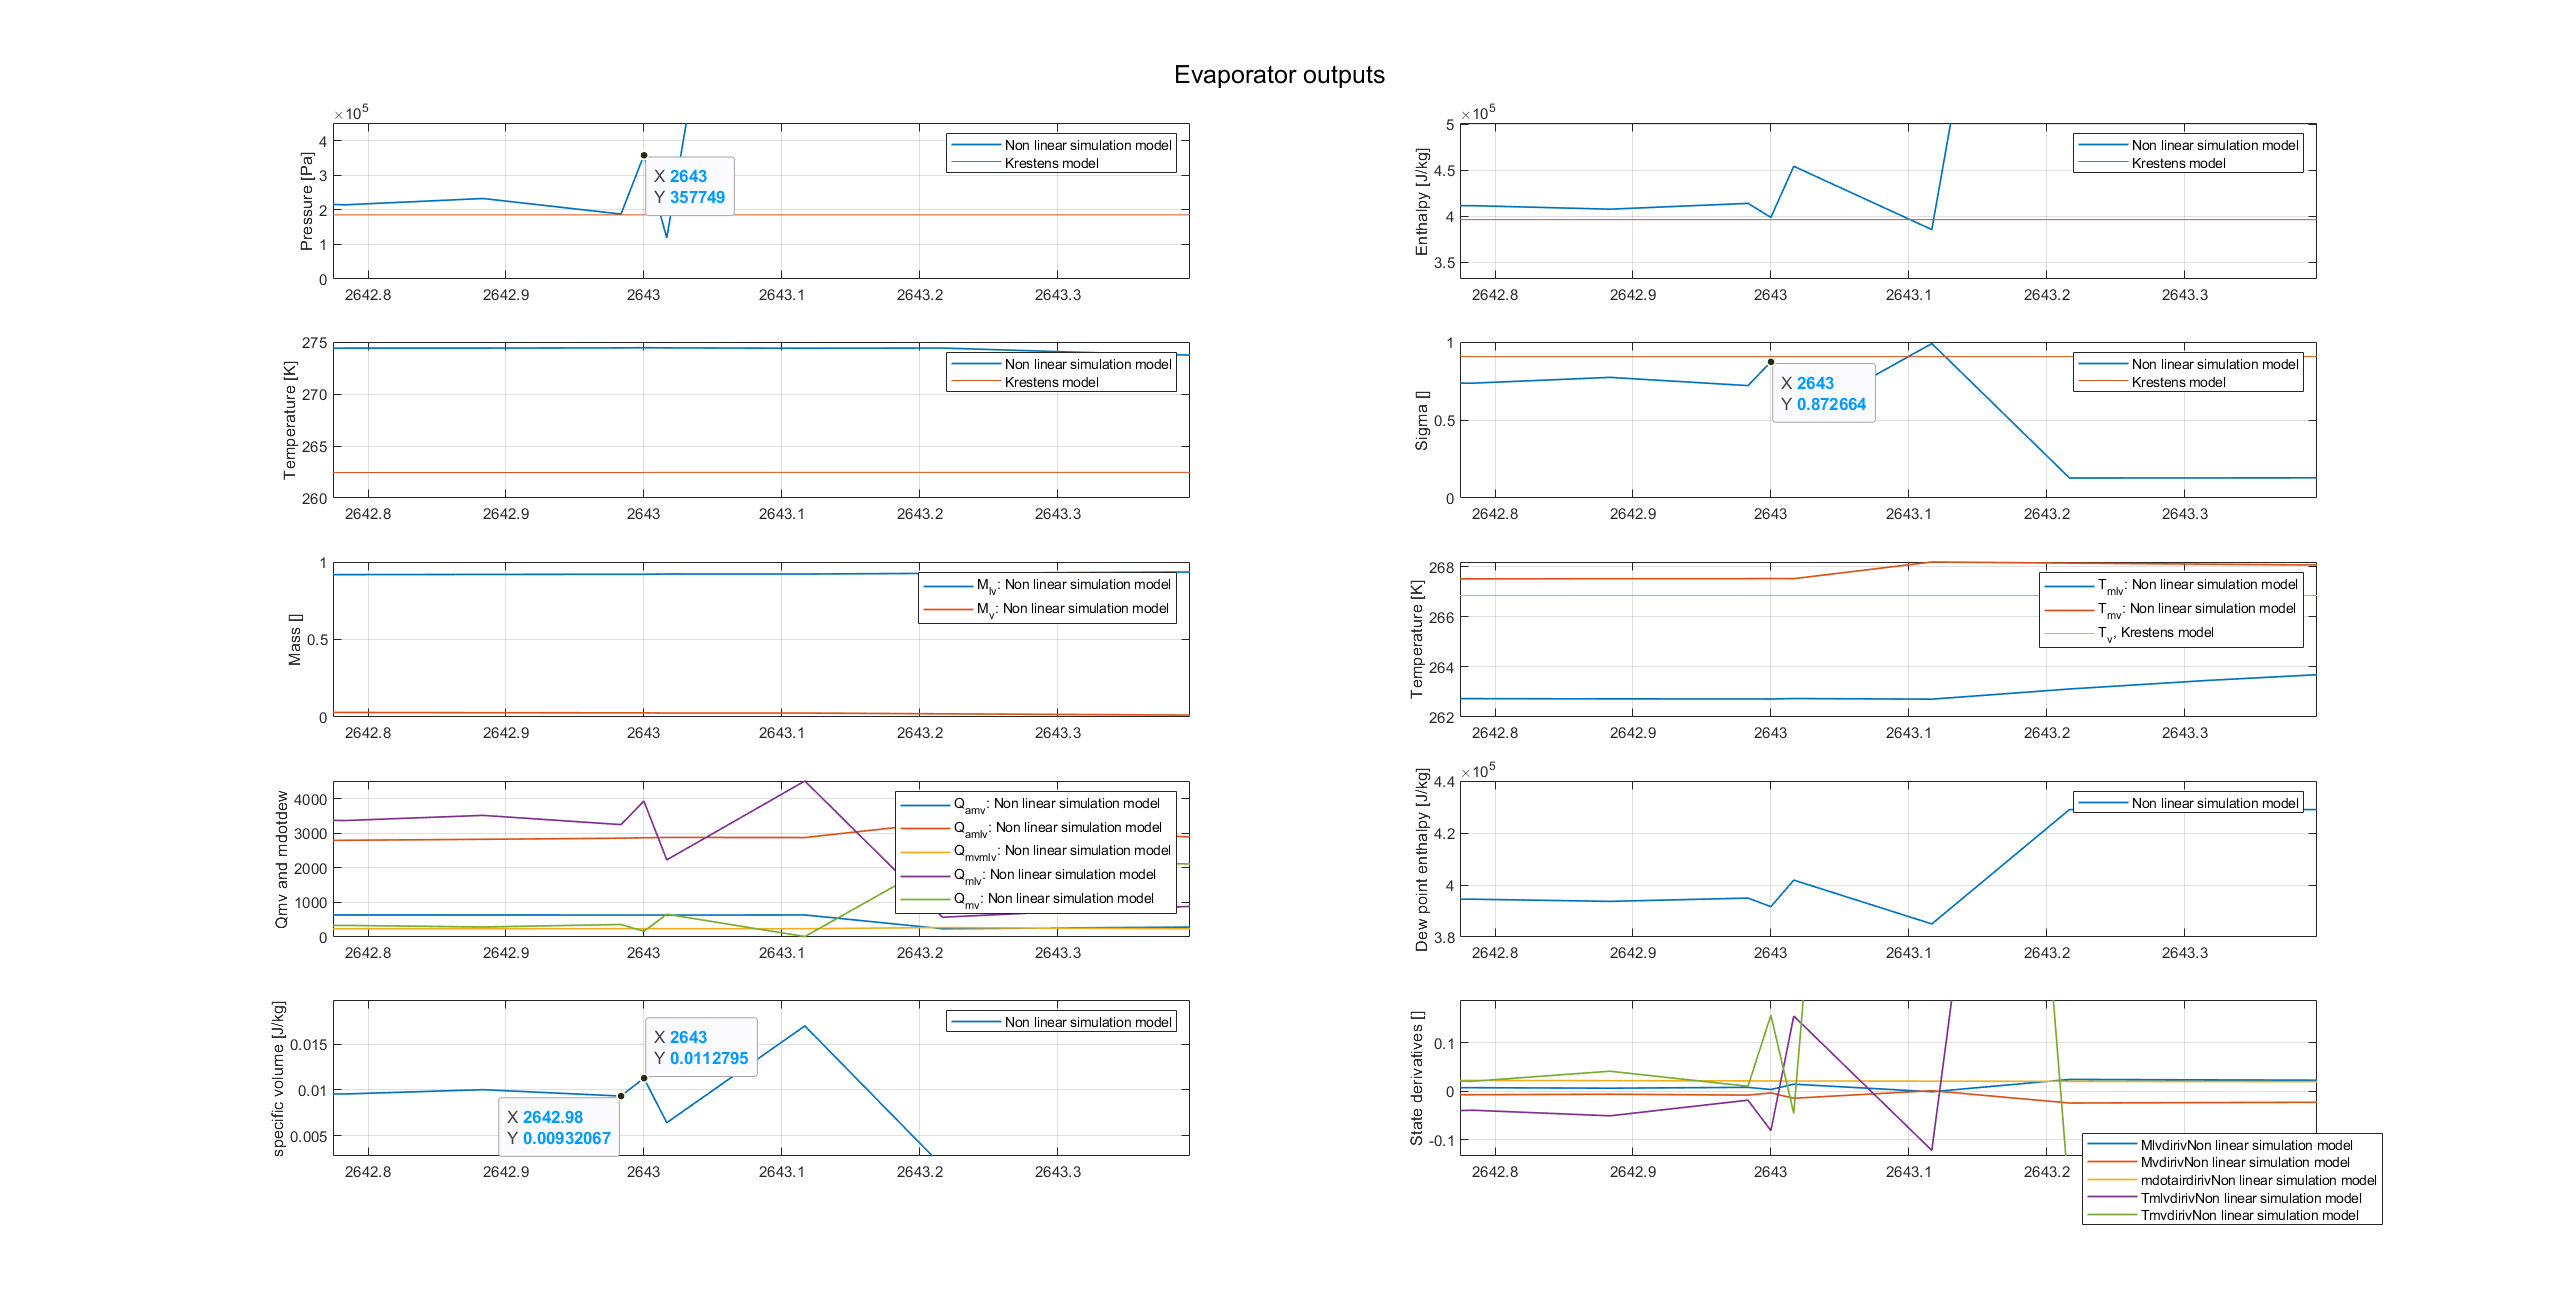
\includegraphics[width=2.1\textwidth]{Tests/Evapo_test1/plot_unstable_zoomed.png}
%	\caption{Zoomed version of \cref{fig:evapotest_plot1}}
%	\label{fig:evapotest_plot2}
%\end{figure}
%In \cref{fig:evapotest_plot2} is a zoom around time t = 2643 s where the simulation proves to start be unstable. From debugging, a sense of a positive feedback loop between look up table from the specific volume and the pressure was assumed. This was the root of the idea of setting $ p_{out} = p_{in} $
%
%\begin{figure}[h]
%	\centering
%	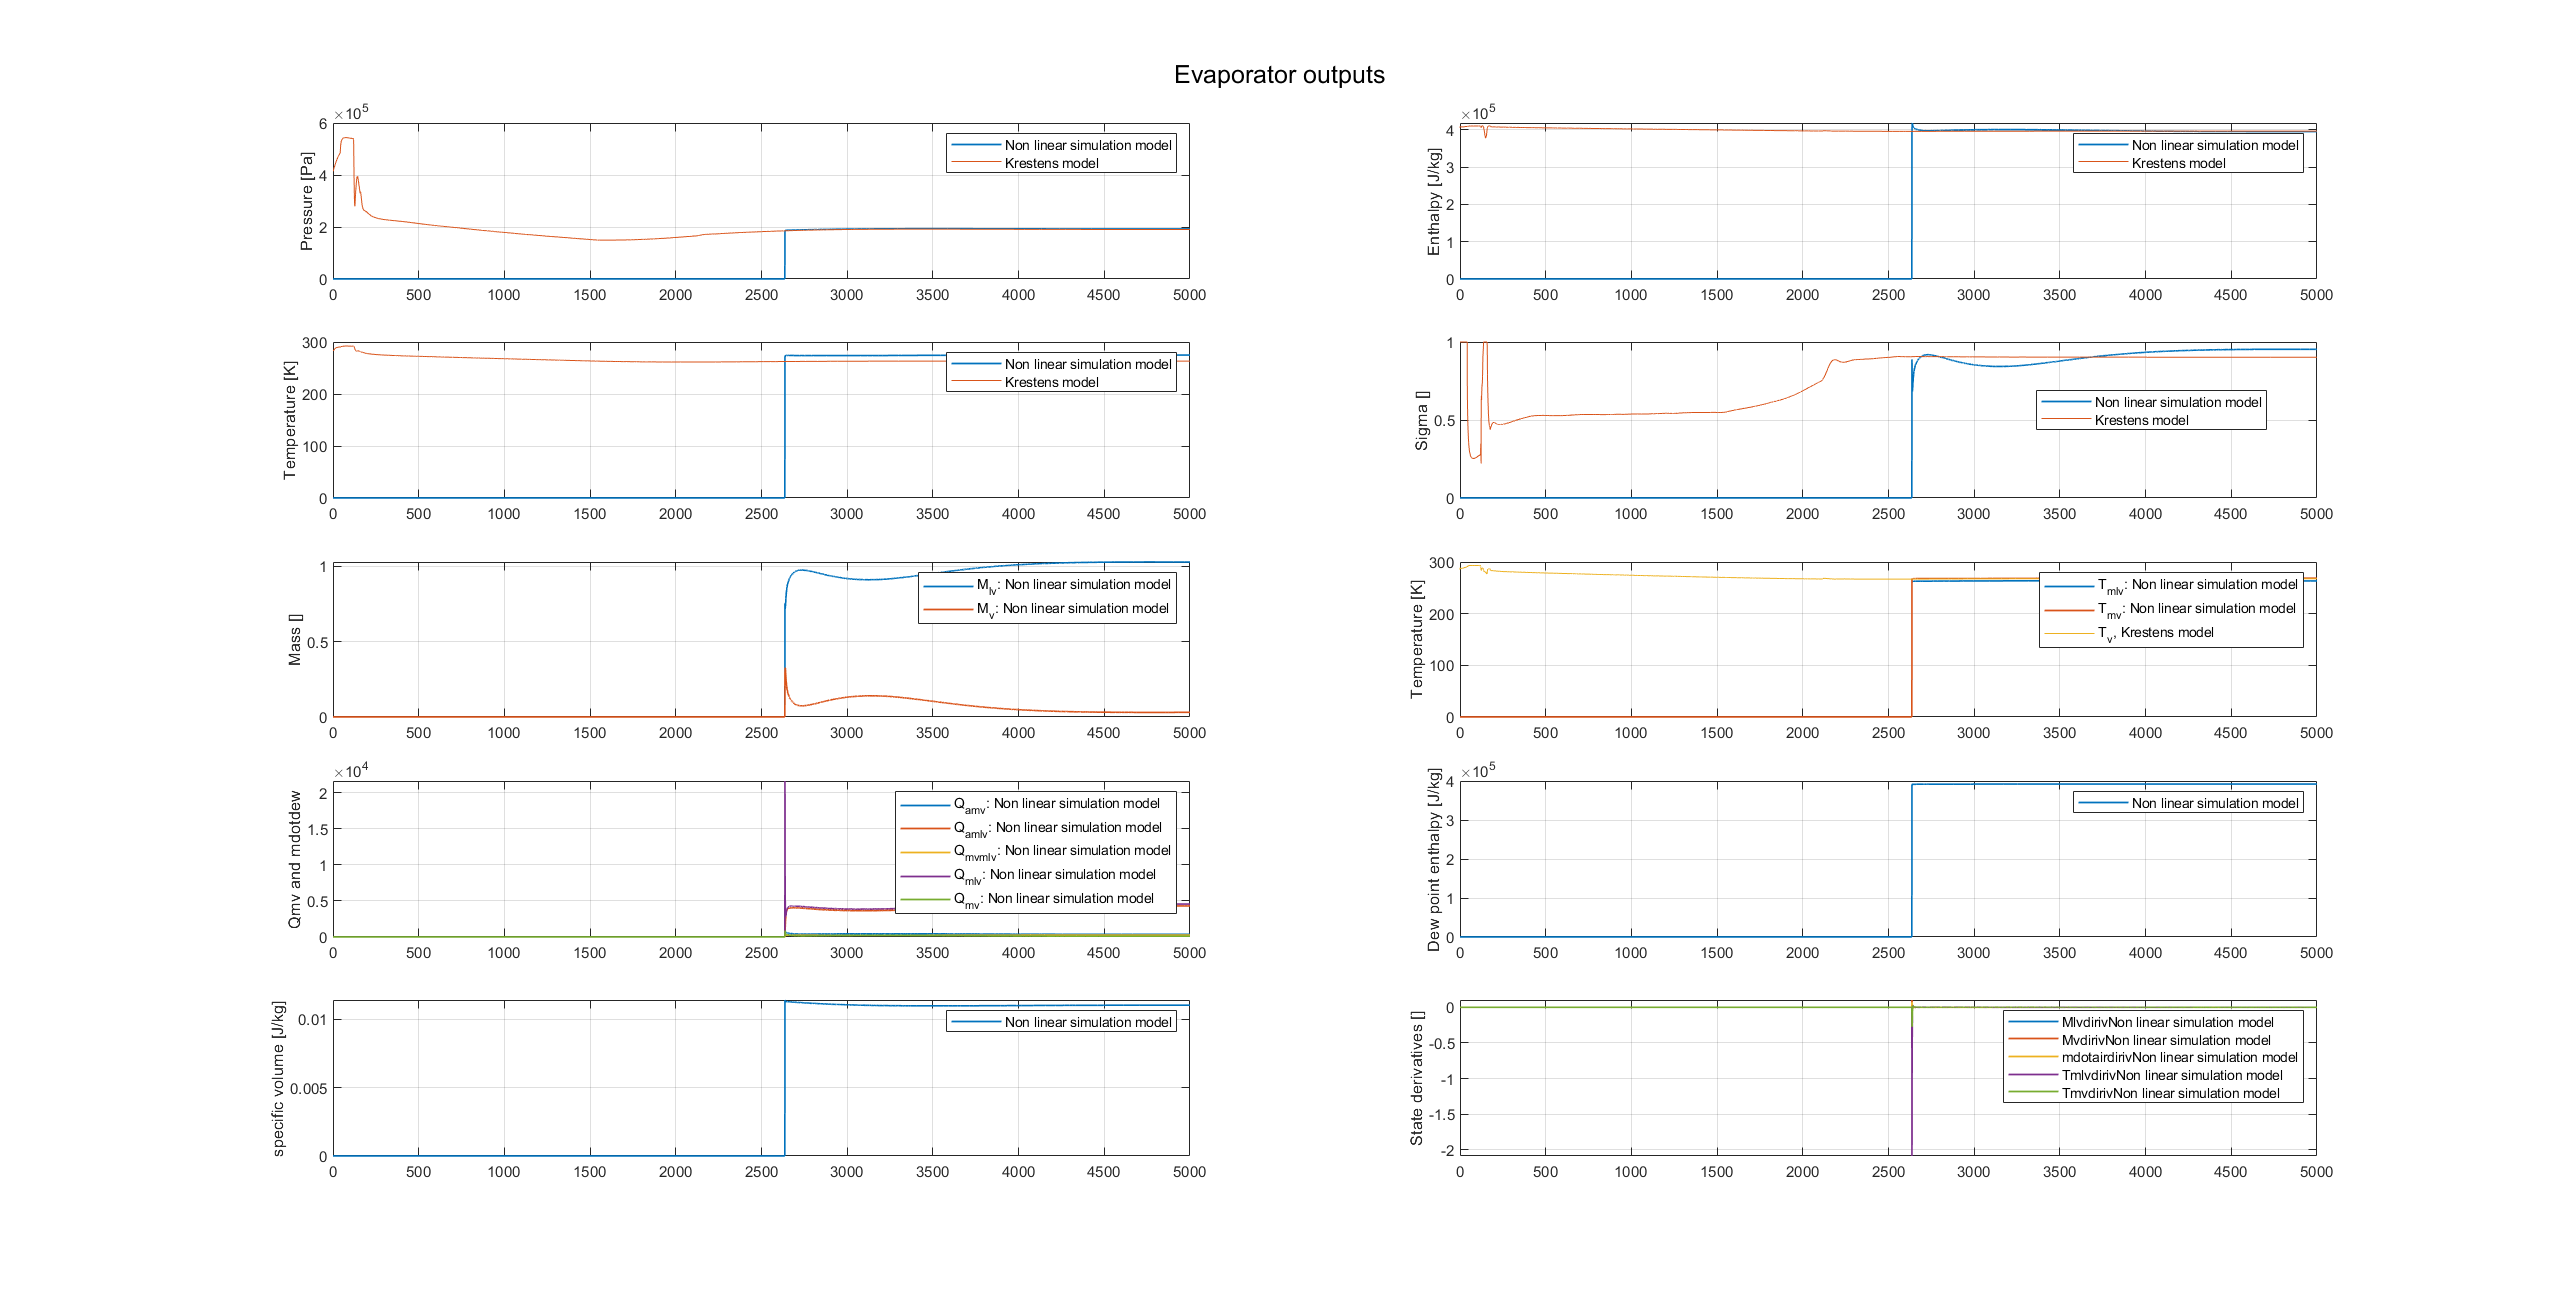
\includegraphics[width=2.1\textwidth]{Tests/Evapo_test1/plot_stable.png}
%	\caption{Simulation with $ p_{out} = p_{in} $}
%	\label{fig:evapotest_plot3}
%\end{figure}
%
%In \cref{fig:evapotest_plot3} where the output pressure is now equal to the input pressure, the behavior is much better, and for this reason we make the assumption that the output pressure is equal to the input pressure.
%
%\clearpage
\subsubsection*{Sources of error and insecurities}
